%% Computers & Operations Research (Elsevier) skeleton.
%% Venue changed from Applied Intelligence 2026-09-11; see the v2 drafts for the
%% section bodies that go here. NOT YET COMPILED -- no local TeX installation;
%% compile on Overleaf, where elsarticle.cls ships by default.
%%
%% Key differences from the svjour3 version this replaces:
%%   - frontmatter block instead of \maketitle + \institute
%%   - theorem environments must be declared HERE (svjour3 predefined them)
%%   - \journalname, \titlerunning, \smartqed all removed (Springer-only)
%%   - bibliography style elsarticle-num instead of spmpsci

\documentclass[preprint,12pt]{elsarticle}

\usepackage{amsmath,amssymb,amsfonts}
\usepackage{amsthm}  % elsarticle has no proof environment; svjour3 provided one
\usepackage{graphicx}
\usepackage{textcomp}
\usepackage{xcolor}
\usepackage{algorithm}
\usepackage{algpseudocode}
\usepackage{booktabs}
\usepackage{multirow}
\usepackage{adjustbox}
\usepackage{float}
\usepackage{bm}
\usepackage{url}

%% elsarticle does NOT predefine these -- svjour3 did, which is why the
%% Springer version carried a comment warning against redeclaring them.
\newtheorem{proposition}{Proposition}
\newtheorem{lemma}{Lemma}
\newtheorem{corollary}{Corollary}
\newtheorem{remark}{Remark}
\newtheorem{definition}{Definition}

\journal{Computers \& Operations Research}

\begin{document}

\begin{frontmatter}

\title{Learning When to Fire: A Minimal-Learning Framework for\\
Dynamic Weapon-Target Assignment}

%% Author block. NOTE: a third author may be added -- an optimization
%% collaborator is being approached to strengthen the exact-method baseline
%% (Section~\ref{sec:results}). Do not finalize the author list or the
%% credit statement until that is settled.
\author[intel]{Jaejin Lee\corref{cor1}}
\ead{jaejin.lee@intel.com}
\cortext[cor1]{Corresponding author.}

\author[asu]{George Runger}
\ead{george.runger@asu.edu}

\address[intel]{Intel Corporation, Chandler, AZ 85226, USA}
\address[asu]{School of Computing and Augmented Intelligence, Arizona State University, Tempe, AZ 85281, USA}

\begin{abstract}
The Dynamic Weapon-Target Assignment Problem (DWTA) asks, at every stage of
an engagement, which weapons should fire and what each should engage, subject
to reload times, ammunition limits, and target availability windows. Learned
approaches typically ask a policy to produce both. We show that only the first
needs learning.

Given the set of weapons firing at a stage, assigning targets among them is
monotone submodular maximization under a partition matroid, and assigning
many-to-one by each weapon's exact marginal value attains at least half the
stage optimum with no learned parameters. The guarantee holds for any firing
set, including one produced by all weapons deciding at once, so the contention
that communication layers and conflict handlers exist to resolve never arises,
and our architecture has neither. Deciding which weapons fire admits no such
treatment: holding fire is worth nothing within a stage and everything across
stages, and we prove that any rule optimizing the current stage can destroy an
arbitrarily small fraction of what an optimal policy destroys.

We therefore learn that decision and nothing else, one Bernoulli parameter per
weapon per stage, delegating assignment to the greedy rule and schedule
revision to a fixed local search that cannot degrade a schedule. Trained only
on instances of 5 to 7 weapons, targets and stages, the framework generalizes
zero-shot to 70 weapons, 100 targets and 15 stages, where it lowers the mean
objective 14.9\% below the strongest learned baseline while running 2.3 times
faster.
%% Keywords live in the skeleton's \begin{keyword} block (elsarticle style),
%% NOT here -- \keywords is a Springer command and is undefined in elsarticle.
\end{abstract}

\begin{keyword}
reinforcement learning \sep combinatorial optimization \sep submodular maximization
\sep local search \sep dynamic weapon-target assignment \sep approximation guarantees
\end{keyword}

\end{frontmatter}

%% \input rather than \include: \include forces a page break before and
%% after every section, which a journal manuscript should not have.
\section{Introduction}
\label{sec:introduction}

%% Introduction, finalized 2026-09-13 after a full line-by-line editing pass
%% with the user. MOVES 1-3 are reproduced here too (previously pulled from
%% BReRLA_manuscript.tex 699-708) so the whole section lives in one file;
%% assemble.py's carry-over of those lines is now redundant but harmless.

The weapon-target assignment problem (WTA), first formalized by Manne in
1958~\cite{manne1958target}, remains an active research problem
today~\cite{ahuja2007exact} because of its continued relevance to modern
defense scenarios. WTA and its variants allocate weapons to targets to
minimize the targets' remaining values after engagement, and the problem is
known to be NP-hard even in its original static, single-stage
form~\cite{lloyd1986weapons}.

The dynamic variant studied here (DWTA) adds four features that make the
model more operationally realistic: (1) multiple engagement stages, (2)
weapon reload times, (3) ammunition limits, and (4) windows during which a
target can be engaged. Given the urgent and time-critical nature of
battlefield situations, the solution method itself must also be fast.

Existing methods are slow in different ways. Exact methods guarantee
optimality but are limited to small instances, making them impractical for
repeated use at every stage for realistically sized
problems~\cite{ahuja2007exact,kline2019weapon}. Heuristics are fast, but each
is typically designed around a specific set of constraints and does not
readily transfer to other settings~\cite{kolitz1988analysis,lee2003genetic}.
Learning-based approaches have been proposed to close this gap, but most
remain narrower in scope. Prior reinforcement learning methods target the
static problem, fix their network size to a particular instance size, or,
when they do scale, assign weapons one at a time, causing computational cost
to grow with the number of
weapons~\cite{na2023weapon,gaudet2023,wu2022dynamic,yoontransformer}.

Unlike single-stage (static) WTA, a DWTA engagement requires each weapon to
make two distinct decisions. First, it must decide whether to fire or reserve
its ammunition for a future engagement. This is a strategic participation
decision. Second, if it fires, it must decide which target to engage. Prior
learned approaches typically ask a single policy to make both decisions,
producing either a target assignment or a decision to skip firing for each
weapon within a stage~\cite{na2023weapon,gaudet2023,yoontransformer}. This is
consistent with the standard design in neural combinatorial
optimization~\cite{kool2018attention,kwon2020pomo}, but it requires the
policy to learn two heterogeneous decisions, which makes the learning 
more difficult. The two decisions are fundamentally different. Target
assignment can be determined from information already known at the current
stage, such as remaining target values, kill probabilities, and current
engagement legality. In contrast, whether to fire depends on the consequences
of preserving ammunition for future stages, which have not yet occurred.
Treating both decisions as a single learning problem obscures this
distinction, and we show that it comes at a measurable cost.

Our claim is that only one of these two decisions needs to be learned. Once
the set of firing weapons is known, their assignment to targets can be solved
directly: a simple greedy rule on marginal value, requiring no training or
learned parameters, provably achieves at least half of the best possible assignment
value (Proposition~\ref{prop:auction-half}). Deciding which weapons should
fire admits no equivalent shortcut. Holding fire provides no benefit within
the current stage and pays off only through future engagements, so any rule
based solely on the current stage can be arbitrarily poor. We show that such
a rule can destroy substantially less target value than an optimal policy
would (Proposition~\ref{prop:myopic-gap}). Thus, we train the model whether to fire or hold and, argue that this minimal learning can achieve reasonably good solutions.

We build this idea into a simple system. A graph neural network considers all
weapons and targets jointly and outputs one number per weapon: the
probability that it should fire in the current stage. All weapons are
decided in a single pass rather than one at a time. A greedy marginal-value rule then
assigns the firing weapons to targets, and a lightweight search revisits the
completed schedule by flipping individual fire-or-hold decisions and
retaining only changes that improve the result. Trained on small instances
(5 to 7 weapons, targets, and stages), the policy generalizes without
further training to problems up to ten times larger, reaching 70 weapons,
100 targets, and 15 stages.

The main contributions of this study are summarized as follows:

\begin{itemize}
\item \textbf{A decomposition with a reason for every part}: We split the
per-stage decision in two. Target assignment is decided by a greedy marginal-value rule with
a provable $\tfrac12$ approximation guarantee (Proposition~\ref{prop:auction-half}). It holds even when weapons decide independently and simultaneously
(Remark~\ref{rem:auction-kills-pileon}). Only the fire and hold (participation decision) is learned for each weapon within the stage (Proposition~\ref{prop:myopic-gap}).

\item \textbf{Learning strictly less, and outperforms baselines}: The
policy outputs one Bernoulli parameter per weapon per stage, not a target
distribution. This reduces the mean objective by 14.9\% across twelve
configurations and outperforms every richer alternative we trained.

\item \textbf{A provably safe improvement step}: At inference we flip individual fire-or-hold decisions and keep only those the re-simulated objective confirms. This reduces the mean objective from 0.1219 to 0.1179 at a budget of ten re-simulations and to 0.1155 at thirty, uses no learned parameters, and cannot make a schedule worse at any budget (Proposition~\ref{prop:search-monotone}).

\item \textbf{Simultaneous decisions with no coordination machinery}: All
weapons are decided in a single pass. The assignment guarantee holds for any
firing set, including one produced by weapons deciding independently
(Remark~\ref{rem:auction-kills-pileon}), so the contention that communication
layers and conflict handlers exist to resolve never arises. Adding
weapon-to-weapon attention under an identical recipe makes the pipeline
slightly worse and three times less stable across seeds
(Section~\ref{sec:ablation}).

\item \textbf{Rigorous, standardized benchmarking}: Evaluation spans four
size tiers up to $70\times100\times15$ under resource scarcity, against exact solution approach,
a greedy heuristic, the auction alone, a sequential decoder, and other RL approaches such as AM and POMO
baselines~\cite{kool2018attention,kwon2020pomo}, all under an identical
protocol.
\end{itemize}

\section{Related Work}
\label{sec:related}

WTA was introduced by Manne~\cite{manne1958target} and is NP-hard even in its static form~\cite{lloyd1986weapons}. Early approaches made the problem tractable through linearization or assumptions such as identical weapons~\cite{day1966allocating,firstman1960approximating,hodson1971linear,bracken1968selected,denbroeder1959optimum}. Exact methods can now certify optimality for moderate static instances, with specialized branch-and-bound methods reaching instances as large as $80\times80$~\cite{ahuja2007exact}. Their computational cost, however, increases sharply beyond that scale~\cite{johansson2009empirical,kline2019weapon}. Heuristics and metaheuristics~\cite{kolitz1988analysis,lee2002immunity,lee2003efficiently,lee2003genetic,durgut2017artificial,sonuc2017parallel,chang2018solving,metler1990suite} provide faster solutions, but are typically designed around specific constraint structures. These limitations motivate methods that can provide fast and repeatable decisions across large and varying problem instances.

Learning-based methods offer an alternative by shifting computational effort to training and producing subsequent decisions through relatively inexpensive forward passes. However, a learned approach must still determine how much of the decision process should be performed by the network itself. Three design choices are particularly relevant to this question. First, should decisions within a stage be generated sequentially or simultaneously? Second, should the network construct the entire decision or delegate part of it to a classical optimization routine? Third, once a solution has been constructed, should improvement be learned or handled by a fixed search procedure? The following literature is organized around these three choices.

\paragraph{Sequential versus simultaneous decision making.}
Neural combinatorial optimization has predominantly adopted sequential solution construction. Pointer networks and attention-based models construct solutions one element at a time, conditioning each decision on those made previously~\cite{vinyals2015pointer,kool2018attention,kwon2020pomo}. Sequential construction naturally provides coordination among decisions, but requires repeated network evaluations as the number of decision makers increases. Simultaneous decision making removes this sequential computational cost but introduces the need to coordinate independent decisions. Several multi-agent learning approaches address this issue through learned communication. CommNet aggregates and broadcasts learned messages~\cite{sukhbaatar2016commnet}, while TarMAC uses attention to determine which agents should communicate with one another~\cite{das2019tarmac}. Pointer-style architectures have also been used to convert the resulting representations into discrete decisions~\cite{park2021schedulenet}. In vehicle routing, where multiple vehicles may compete for the same customer, PARCO introduces a learned priority-based mechanism to resolve such conflicts~\cite{parco2024}.

Multi-agent reinforcement learning has more commonly retained sequential action generation. The multi-agent advantage decomposition framework expresses the joint advantage as a sum of per-agent advantages conditioned on the actions of preceding agents, enabling sequential policy optimization with monotonic improvement guarantees. HATRPO and HAPPO build directly on this framework~\cite{kuba2022trust}, while the Multi-Agent Transformer incorporates the sequential structure through autoregressive action generation~\cite{wen2022mat}. Subsequent work has also considered how the ordering of agents should be selected~\cite{wen2022mat}. These approaches highlight the importance of coordination when multiple agents make discrete resource-allocation decisions. Our framework reaches the same end by a different route: rather than ordering the agents, it removes target selection from them entirely, and the assignment guarantee of Proposition~\ref{prop:auction-half} then holds however the participating agents were chosen.

\paragraph{Learning versus classical decision mechanisms.}
The second design choice concerns whether the network should produce the entire decision or delegate part of it to a classical procedure. Such hybrid designs have been explored in several learning-based optimization settings. Delarue et al.\ embed an optimization subproblem directly into policy action selection~\cite{delarue2020rl}, while reinforcement learning has also been used to determine bidding values within an auction mechanism~\cite{sun2026grabbing}. Our framework follows this general principle but uses the structure of DWTA to determine where the decision should be divided.

Specifically, the target-assignment component admits a per-stage approximation guarantee: the auction mechanism obtains at least one half of the optimal assignment value (Proposition~\ref{prop:auction-half}). In contrast, the participation decision cannot be assigned an analogous per-stage guarantee, because a decision based only on current-stage information can be arbitrarily suboptimal when future engagements are considered (Proposition~\ref{prop:myopic-gap}). We therefore delegate target assignment to the classical auction mechanism while learning the participation decision. The decomposition is thus motivated by the properties that can be established for each component rather than solely by implementation convenience.

This decomposition also changes the role of simultaneous decision making. Existing communication and sequential-decoding methods primarily address coordination among agents competing for resources. In our framework, the neural policy does not select targets; instead, it produces a participation decision for each weapon, after which the auction determines the corresponding assignment from the stage state. Consequently, the target preferences that produce the $\Theta(1/M)$ worst-case loss in simultaneous target selection are not used by the policy (Remark~\ref{rem:auction-kills-pileon}). The coordination problem associated with simultaneous target selection is therefore removed rather than learned around. This allows simultaneous participation decisions while retaining the assignment guarantee provided by the auction.

\paragraph{Learning versus fixed improvement.}
A third line of work focuses on improving an already constructed solution rather than learning the complete construction process. Neural local-rewriting methods repeatedly propose modifications to an existing solution and accept changes according to an improvement criterion~\cite{chen2019rewriter}. Related approaches include learned improvement heuristics for routing~\cite{wu2021improvement} and dual-aspect representations for local improvement~\cite{ma2021dact}. Zhang, Hu, and Zhao use a similar pipeline for vehicle routing with time windows, combining an attention-based construction policy with classical large-neighbourhood search~\cite{zhang2025vrptw}.

We investigated the same idea for DWTA by training a schedule-editing policy that scores every stage-weapon slot and selects the highest-scoring slot to flip. In our experiments, the learned selector accounted for only 24\% of the observed improvement, while uniformly random slot selection under the same re-simulation budget and acceptance rule reproduced the remaining 76\%. Under a strictly improving acceptance rule, the learned ordering was even worse than random selection. This result concerns the specific edit operator used in our framework rather than the cited methods, whose problem settings and operators differ. In our case, the edit space consists of a single binary participation decision for each stage-weapon pair, leaving relatively little additional structure for a learned selector to exploit. These observations motivate the use of a fixed hill-climbing procedure rather than a second learned network.

\paragraph{Reinforcement learning for weapon-target assignment.}
The reinforcement-learning literature on WTA provides a more direct comparison with our framework. Early neural formulations date to Wacholder~\cite{wacholder1989neural}. More recent approaches can be distinguished according to whether they address dynamic settings, support variable problem sizes, and incorporate the operational constraints relevant to DWTA. Table~\ref{tab:related} summarizes these characteristics.

For static WTA, several approaches either use architectures whose dimensions depend on the instance size~\cite{meng2021deep,shin2020mean,gaudet2023} or achieve size-agnostic architectures by simplifying the operational setting, such as omitting relevant constraints or assuming identical weapons~\cite{luo2021learning,na2023weapon,vinyals2015pointer}. Dynamic approaches similarly retain at least one of these limitations, including size-fixed architectures~\cite{wu2022dynamic}, simplified objectives based on identical agents~\cite{hu2024}, or receding-horizon decompositions that do not learn a cross-stage policy~\cite{zhang2020efficient,zhang2020dynamic}.

Closest to our work, Yoon, Lee, and Cho~\cite{yoontransformer} consider scalable dynamic WTA using a transformer-based policy. Our approach differs in two main respects. First, the policy predicts participation rather than directly selecting a target. Second, we provide a theoretical characterization of when delegating target assignment to a fixed rule is safe (Section~\ref{sec:auction}). More recently, Oh et al.~\cite{oh2026combat} combine graph neural networks with reinforcement learning for dynamic WTA, using a graph-attention policy trained with PPO under a partially observable formulation and evaluating naval and ground scenarios against heuristic and metaheuristic baselines. Their emphasis is on scenario realism through the OODA decision cycle, whereas our focus is on decomposing the per-stage decision into a learned participation policy and a classical assignment mechanism with a per-stage approximation guarantee. We further evaluate this framework against an exact solver and neural construction baselines.

Overall, existing reinforcement-learning approaches to WTA generally assume that the learned policy directly produces the complete per-stage assignment decision. Our framework instead separates the decision into participation and target assignment, learns only the component that requires cross-stage reasoning, and delegates the remaining component to a classical mechanism with a provable per-stage guarantee.

%% NOTE 2026-08-23: JDMS full text inaccessible (SAGE 403); published abstract (framework "ARFA") does not
%% disambiguate sequential vs simultaneous decoding. The single-sequential-policy characterization stands on
%% the co-author's (J. Lee's) own description in this manuscript's Method overview; final confirmation at
%% proof stage costs one glance at the published paper. Bib entry updated with year 2025 + doi.
%% CITATION STATUS 2026-08-23: (a) Oh et al. IEEE T-Cyb verified via Crossref (vol. 56, no. 2, pp. 631-643, 2026,
%% doi 10.1109/TCYB.2025.3610606; TechRxiv preprint 10.36227/techrxiv.171084935.57702557) and cited in prose above
%% using only abstract-verifiable claims (DWTA, GNN+PPO, POMDP, OODA, heuristic/metaheuristic baselines). NOT added
%% to Table~\ref{tab:related}: the sequential-vs-parallel and constraint axes could not be verified (full text
%% paywalled, preprint mirrors blocked) and must not be assumed. (b) the "Control Theory & Applications 2025" item
%% previously noted here could not be located under that title in Crossref or web search: it appears to have been
%% a garbled duplicate of (a); dropped.

\begin{table}[htbp]
\centering
\small
\caption{Reinforcement-learning approaches to weapon-target assignment along the axes that position this work.}
\label{tab:related}
\begin{tabular}{l|ccc}
\hline
\textbf{Method} & \textbf{Dynamic} & \textbf{Size-agn.} & \textbf{Parallel dec.} \\ \hline
Meng et al.~\cite{meng2021deep} & -- & -- & -- \\
Shin et al.~\cite{shin2020mean} & -- & -- & -- \\
Luo et al.~\cite{luo2021learning} & -- & \checkmark & -- \\
Na \& Choi~\cite{na2023weapon} & -- & \checkmark & -- \\
Gaudet et al.~\cite{gaudet2023} & -- & -- & -- \\
Wu et al.~\cite{wu2022dynamic} & \checkmark & -- & -- \\
Hu et al.~\cite{hu2024} & \checkmark & \checkmark & -- \\
Yoon et al.~\cite{yoontransformer} & \checkmark & \checkmark & -- \\ \hline
\textbf{This work} & \checkmark & \checkmark & \checkmark \\ \hline
\end{tabular}
\end{table}

\section{Problem Formulation}
\label{sec:problem}

DWTA extends the static problem over a horizon of discrete stages
$t = 1, 2, \ldots, T$. At each stage, every weapon either fires one round at a
single target or holds. A weapon that fires becomes unavailable for a fixed
number of stages, spends one round of a finite magazine, and may only engage
targets that are currently exposed. The
static problem has none of these features, and they are what make the choice
to hold fire meaningful: a round spent now is a round unavailable later.

The objective is to minimize the total value of the targets that survive the
engagement. The model rests on the following assumptions.

\begin{itemize}
    \item A weapon fires at most one round per stage, at a single target.
    Several weapons may engage the same target in the same stage.
    \item Weapon $m$ requires a reload time $D_m$. After firing, it cannot
    fire again for $D_m$ stages.
    \item Weapon $m$ carries $A_m$ rounds for the entire horizon.
    \item Target $n$ is exposed only during its time window $TW_n$, which runs
    from $t_{n,\text{start}}$ to $t_{n,\text{end}}$, and cannot be engaged
    outside it.
    \item A hit by weapon $m$ removes a fixed proportion $P_{m,n}$ of the
    remaining value of target $n$. Hits therefore compound multiplicatively,
    and each additional hit on the same target is worth less than the one
    before it.
\end{itemize}

Table~\ref{tab:notation} lists the notation. The two state variables
$w_{m,t}$ and $a_{m,t}$ track reload and ammunition from stage to stage.

\begin{table}[H]
\centering
\small
\caption{Notation for the mathematical model.}
\label{tab:notation}
\begin{tabular}{lp{6.5cm}}
\hline
\textbf{Sets} & \\
$M$ & Set of weapons, indexed by $m = 1, \ldots, M$ \\
$N$ & Set of targets, indexed by $n = 1, \ldots, N$ \\
$T$ & Set of stages, indexed by $t = 1, \ldots, T$ \\
\hline
\textbf{Parameters} & \\
$V_n$ & Initial value of target $n$ \\
$D_m$ & Reload time of weapon $m$, in stages \\
$A_m$ & Rounds available to weapon $m$ over the horizon \\
$TW_n$ & Time window during which target $n$ is exposed \\
$P_{m,n}$ & Proportion of target $n$'s remaining value removed by a hit from weapon $m$ \\
\hline
\textbf{Decision Variables} & \\
$x_{m,n,t}$ & $1$ if weapon $m$ engages target $n$ at stage $t$, $0$ otherwise \\
$w_{m,t}$ & Stages remaining before weapon $m$ is ready again \\
$a_{m,t}$ & Rounds remaining to weapon $m$ at stage $t$ \\
\hline
\end{tabular}
\end{table}

Each hit on target $n$ scales its remaining value by $(1 - P_{m,n})$, so the
value surviving the engagement is a product over all hits the target
receives, and the objective is
\begin{equation}\label{eq:objective_function}
    \min \sum_{n=1}^{N} V_{n} \prod_{t=1}^{T} \prod_{m=1}^{M} (1 - P_{m,n})^{x_{m,n,t}},
\end{equation}
subject to the assumptions above. \ref{app:model} states them as constraints
and gives the full nonlinear integer program.

At a given stage, the reload, ammunition and time-window constraints leave
each weapon a set of targets it may engage,
\begin{equation}\label{eq:legal-set}
    \mathcal{L}_{m,t} = \{\, n : t \in TW_n \,\} \quad \text{if } w_{m,t} = 0 \text{ and } a_{m,t} \geq 1, \qquad \mathcal{L}_{m,t} = \emptyset \ \text{otherwise}.
\end{equation}
This set is what the policy of Section~\ref{sec:method} is masked to.

The objective is nonlinear in the assignment variables, and the reload and
ammunition state couples the stages: a round fired at stage $t$ removes value
now and removes an option later. That coupling is the part of the problem no
single-stage rule can reason about, and Section~\ref{sec:participation-theory} makes the
consequence precise.

\section{Markov Decision Process Formulation}
\label{sec:mdp}

% Formulations of this problem conventionally give the policy the full
% per-stage decision: which target, if any, each weapon engages. Section~\ref{sec:auction} shows that half of this decision, target assignment given a set of firing weapons, admits a mechanism with a
% provable approximation guarantee and no learning at all.
We define the MDP so that the policy is only ever asked whether each weapon fires this stage. An MDP, $\mathcal{M}$, is represented as a 5-tuple:
\begin{equation}
\mathcal{M} = (\mathcal{S}, \mathcal{A}, \mathcal{T}, R, \gamma)
\end{equation}
where $\mathcal{S}$ is the state space, $\mathcal{A}$ the action space,
$\mathcal{T}$ the transition kernel, $R$ the reward function, and $\gamma$
the discount factor.

\begin{itemize}
\item \textbf{State ($s_t$)}: for every (weapon, target) pair, the
nine quantities
\begin{equation}
\label{eq:state}
s_t = [u_t;\, v_t;\, d_t;\, r_t;\, \alpha_t;\, f_t;\, ws;\, we;\, p] \in \mathbb{R}^9,
\end{equation}
namely weapon readiness $u_t$, remaining target value $v_t$, remaining reload
time $d_t$, remaining time to horizon $r_t$, remaining ammunition $\alpha_t$,
cumulative hits on the target $f_t$, the window bounds $ws$ and $we$, and the
damage rate $p = P_{m,n}$. Section~\ref{sec:encoding} encodes these as a
heterogeneous graph rather than as $M \times N$ independent vectors.

\item \textbf{Action ($a_t$)}: a \emph{binary} per-weapon participation
decision,
\begin{equation}
\label{eq:binary-action}
a_t = (a_{1,t}, \ldots, a_{M,t}) \in \{0,1\}^M, \qquad a_{m,t} = 1 \iff m \text{ fires at } t,
\end{equation}
rather than a choice of target. This is the entire output the policy is
responsible for: $2^M$ joint actions per stage, against the
$\prod_m (|\mathcal{L}_{m,t}|+1)$ a target-selecting formulation would have to choose from.

\item \textbf{Transition}: given $a_t$, the environment (not the policy)
determines the realized engagement. The set of firing weapons
$F_t = \{m : a_{m,t}=1\}$ is passed to a fixed assignment routine
\begin{equation}
\label{eq:auction-call}
x_t = \textsc{Assign}(F_t, s_t),
\end{equation}
which gives each $m \in F_t$ one target, choosing greedily by the value a
shot would destroy at the current state. It is deterministic, has no learned
parameters, and is defined in full in Section~\ref{sec:auction}. A weapon in
$F_t$ with no legal target is a no-op regardless of $a_{m,t}$. The transition
$\mathcal{T}(s_{t+1} \mid s_t, a_t)$ is therefore deterministic once $a_t$
is fixed, but it is not simply ``apply $a_t$'': it composes the policy's
binary decision with the fixed assignment rule.

\item \textbf{Reward}:
\begin{equation}
R(s_{t+1} \mid s_t, a_t) = \frac{C(s_t) - C(s_{t+1})}{C(s_0)},
\end{equation}
where $C(s_t)$ is the sum of remaining target values at $s_t$, realized
through the assigned engagement rather than a directly-specified one.
\end{itemize}

This factoring of the decision, learn participation and delegate assignment,
is what Section~\ref{sec:method} implements, and what
Section~\ref{sec:participation-theory}'s myopic-gap proposition argues cannot be
undone: the assignment rule alone, applied to \emph{every} weapon with a
positive marginal value each stage, is a valid (if unlearned) participation
rule, and
Proposition~\ref{prop:myopic-gap} shows it can be arbitrarily far from
optimal. The gap between that myopic rule and the optimal one is exactly
what Eq.~\eqref{eq:binary-action}'s policy is trained to close.

\section{Proposed Method}
\label{sec:method}

The proposed framework embeds the MDP state using a
GNN~\cite{gilmer2017neural}, and decides fire or hold for every weapon. The
greedy marginal-value rule assigns targets to the firing
weapons. A fixed local search then revises the completed schedule. Only the
fire-or-hold decision is learned. Fig.~\ref{fig:overall} shows the pipeline
and Algorithm~\ref{alg:scope} states it precisely.

%% Figure generated by paper/make_overall_figure.py (matplotlib). Edit that
%% script and re-run it rather than editing the PNG. Grayscale by design.
\begin{figure}[htbp]
  \centering
  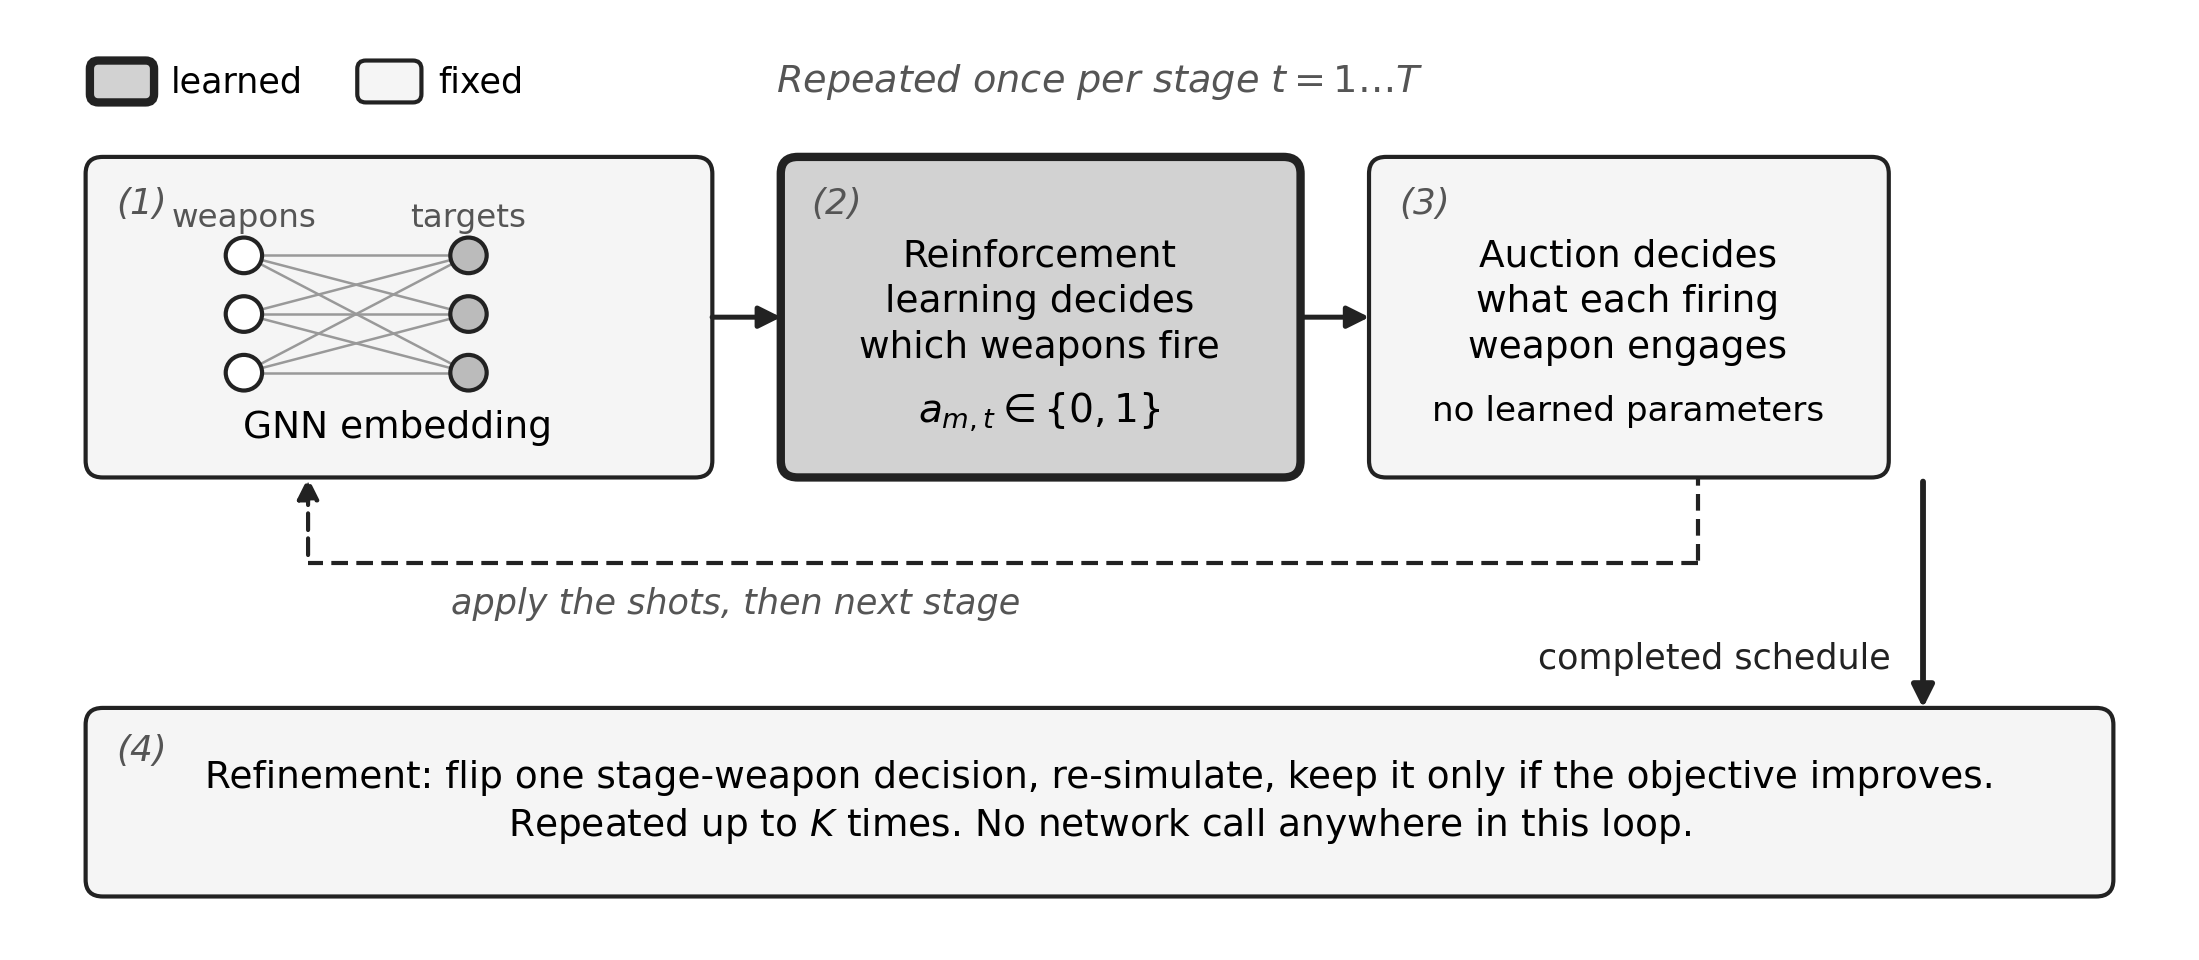
\includegraphics[width=\columnwidth]{figure/Overall.png}
  \caption{The pipeline, corresponding step for step to
  Algorithm~\ref{alg:scope}. Border weight marks the one learned box: the
  policy emits one bit per weapon and nothing else.}
  \label{fig:overall}
\end{figure}

\begin{algorithm}[htbp]
\caption{Inference: construction followed by fixed local search}
\label{alg:scope}
\begin{algorithmic}[1]
\Require instance $(V, P, A, D, TW)$; participation policy $\pi_\theta$; edit budget $K$
\Ensure feasible schedule
\Statex \textbf{Construction}
\State $s_1 \gets$ initial state
\For{$t = 1$ \textbf{to} $T$}
  \State $H^{\text{wpn}}, H^{\text{tgt}}, H^{\text{edge}} \gets \textsc{Encode}(s_t)$ \Comment{$L$ message-passing rounds, Sec.~\ref{sec:encoding}}
  \State $a_{m,t} \gets \mathbb{1}\!\left[\pi_m(\text{fire}\mid s_t) > \tfrac12\right]$ for all $m$ \Comment{one forward pass, Eq.~\eqref{eq:fire-prob}}
  \State $F_t \gets \{m : a_{m,t} = 1\}$
  \State $x_t \gets \textsc{Assign}(F_t, s_t)$ \Comment{many-to-one, Sec.~\ref{sec:auction}}
  \State $s_{t+1} \gets \textsc{Step}(s_t, x_t)$
\EndFor
\State $\phi \gets \bm{0}$; \; $\mathit{tried} \gets \emptyset$; \; $J^\star \gets J(\phi)$
\Statex \textbf{Fixed local search (Sec.~\ref{sec:local-search})}
\For{$k = 1$ \textbf{to} $K$}
  \If{$\mathit{tried}$ covers every slot} \textbf{break} \Comment{1-flip local optimum} \EndIf
  \State draw $(t^\ast\!, m^\ast)$ uniformly from the untried slots
  \State $\phi' \gets \phi$ with $\phi'_{t^\ast\!,m^\ast}$ flipped
  \State $J' \gets J(\phi')$ \Comment{re-simulate: assignment + environment only, no network call}
  \If{$J' < J^\star$}
    \State $\phi \gets \phi'$; \; $J^\star \gets J'$; \; $\mathit{tried} \gets \emptyset$
  \Else
    \State $\mathit{tried} \gets \mathit{tried} \cup \{(t^\ast\!,m^\ast)\}$
  \EndIf
\EndFor
\State \Return schedule induced by $\phi$
\end{algorithmic}
\end{algorithm}

\subsection{Heterogeneous Graph Encoding}
\label{sec:encoding}

Each weapon-target pair state can be represented as a vector in $\mathbb{R}^9$ (Eq.~\eqref{eq:state}). We encode this state with a graph neural network rather than feeding the $M \times N$ vectors to the policy directly, for two reasons. First, only the damage rate $P_{m,n}$ is a property of the pair; the remaining features belong to a weapon or to a target alone, and a graph stores each of them once instead of copying them across all pairs. Second, a graph network has no dimension tied to $M$ or $N$, so one trained model applies to any problem size, which is the property the zero-shot generalization in Section~\ref{sec:results} rests on.
%% Verified 2026-08-23 against common/Dynamic_Instance_generation.py + DWTA_GNN_comm_sinkhorn.py:
%% weapon node = features [ammunition, availability, remaining time, waiting time] = {a_t,u_t,r_t,d_t}.

The graph is bipartite: weapon nodes $\bm{x}_m^{\text{wpn}} \in \mathbb{R}^4$, target nodes $\bm{x}_n^{\text{tgt}} \in \mathbb{R}^4$, and one edge carrying $\bm{x}_{m,n}^{\text{edge}} = P_{m,n}$ for every weapon-target pair. Each node and edge is first projected to a common hidden width $H$:
\begin{equation}
\label{eq:gnn-proj}
\begin{gathered}
\bm{h}_m^{\text{wpn},(0)} = \bm{W}^{\text{wpn}}\bm{x}_m^{\text{wpn}} + \bm{b}^{\text{wpn}}, \qquad
\bm{h}_n^{\text{tgt},(0)} = \bm{W}^{\text{tgt}}\bm{x}_n^{\text{tgt}} + \bm{b}^{\text{tgt}}, \\
\bm{h}_{m,n}^{\text{edge},(0)} = \bm{W}^{\text{edge}}\bm{x}_{m,n}^{\text{edge}} + \bm{b}^{\text{edge}}.
\end{gathered}
\end{equation}
Then $L$ rounds of message passing follow~\cite{gilmer2017neural}. At round $\ell$, each edge is updated from its two endpoint embeddings and its own previous value,
\begin{equation}
\label{eq:gnn-edge}
\bm{h}_{m,n}^{\text{edge},(\ell)} = \tanh\!\left(\bm{W}_e\left[\bm{h}_m^{\text{wpn},(\ell-1)} \,\|\, \bm{h}_n^{\text{tgt},(\ell-1)} \,\|\, \bm{h}_{m,n}^{\text{edge},(\ell-1)}\right]\right),
\end{equation}
and each weapon node aggregates the messages of its incident edges through a GRU,
\begin{equation}
\label{eq:gnn-node}
\begin{aligned}
\bm{\mu}_{m,n}^{(\ell)} &= \bm{W}_w\big[\bm{h}_m^{\text{wpn},(\ell-1)} \,\|\, \bm{h}_n^{\text{tgt},(\ell-1)} \,\|\, \bm{h}_{m,n}^{\text{edge},(\ell)}\big],\\
\bm{h}_m^{\text{wpn},(\ell)} &= \text{GRU}\Big(\textstyle\sum_{n=1}^{N} \bm{\mu}_{m,n}^{(\ell)},\ \bm{h}_m^{\text{wpn},(\ell-1)}\Big),
\end{aligned}
\end{equation}
where $\|$ denotes concatenation. The target update $\bm{h}_n^{\text{tgt},(\ell)}$ is defined analogously, aggregating over all weapons. After $L$ rounds, each weapon embedding $\bm{h}_m^{\text{wpn},(L)}$ reflects the state of the whole battlefield, and each edge embedding $\bm{h}_{m,n}^{\text{edge},(L)}$ carries the pair information that the decoder scores (Section~\ref{sec:parallel-decoder}).


\subsection{Binary Participation Policy}
\label{sec:parallel-decoder}

For each weapon $m$, the policy scores two kinds of options from the encoder
output: firing at each legal target $n \in \mathcal{L}_{m,t}$, and holding,
\begin{equation}
\label{eq:edge-score}
\text{score}_{m,n} = \bm{w}_e^\top \, \text{Res}\big(\bm{h}_{m,n}^{\text{edge},(L)}\big), \quad n \in \mathcal{L}_{m,t},
\end{equation}
\begin{equation}
\label{eq:noop-score}
\text{score}_{m,\text{hold}} = \bm{w}_0^\top \, \text{Res}\!\left(\bm{W}_0\left[\bm{h}_m^{\text{wpn},(L)} \,\|\, \bar{\bm{h}}^{\text{wpn}} \,\|\, \bar{\bm{h}}^{\text{tgt}}\right]\right),
\end{equation}
where $\text{Res}(\cdot)$ is a residual block with layer normalization and
$\bar{\bm{h}}^{\text{wpn}}, \bar{\bm{h}}^{\text{tgt}}$ are the mean embeddings
of all weapons and all targets. A softmax over these scores gives the
probability of holding,
\begin{equation}
\label{eq:hold-prob}
\pi_m(\text{hold} \mid s_t) = \frac{\exp(\text{score}_{m,\text{hold}})}{\exp(\text{score}_{m,\text{hold}}) + \sum_{n \in \mathcal{L}_{m,t}} \exp(\text{score}_{m,n})},
\end{equation}
and the probability of firing is its complement,
\begin{equation}
\label{eq:fire-prob}
p_{m,t} = \pi_m(\text{fire} \mid s_t) = 1 - \pi_m(\text{hold} \mid s_t).
\end{equation}
Which target the firing weapon engages is decided by the assignment step
(Section~\ref{sec:auction}), not by the scores.

All $M$ weapons are scored in one forward pass, and each decision is sampled
independently:
\begin{equation}
\label{eq:bernoulli}
a_{m,t} \sim \text{Bernoulli}(p_{m,t}),
\end{equation}
so the log-probability of the joint action is
\begin{equation}
\log \pi_\theta(a_t \mid s_t) = \sum_{m=1}^M \big[a_{m,t}\log p_{m,t} + (1-a_{m,t})\log(1-p_{m,t})\big].
\end{equation}

\subsection{Target Assignment by Greedy Marginal Value}
\label{sec:auction}

Given the set of firing weapons $F$ at stage $t$, the assignment step gives
each of them one target. The classical assignment problem has a linear
objective and is solved exactly in polynomial
time~\cite{kuhn1955hungarian,burkard2012assignment}. The DWTA stage problem is
many-to-one and its objective is nonlinear, so those methods do not apply
directly. We assign greedily by exact marginal value.

Let $\rho_n^{(t)}$ be the fraction of target $n$'s value that survives into
stage $t$, and let $E_t = \{(m,n) : m \in F,\ (m,n) \text{ feasible at } t\}$.
For a set of assigned pairs $S_t \subseteq E_t$, the value destroyed in the
stage is
\begin{equation}
\label{eq:round-obj}
f_t(S_t) = \sum_{n=1}^N V_n\rho_n^{(t)}\left(1 - \!\!\prod_{m:(m,n)\in S_t}\!\!(1-P_{m,n})\right).
\end{equation}
This objective is monotone submodular~\cite{wang2013weapon}: adding a weapon
to a target never hurts, but helps less when other weapons already engage it.
Each weapon takes at most one pair, which is a partition matroid constraint.
Maximizing such a function is NP-hard~\cite{feige1998threshold}, so we seek an
assignment that is provably good rather than optimal.

If $S_n$ is the set of weapons already assigned to target $n$, the score of
weapon $m$ for target $n$ is its exact marginal value,
\begin{equation}
\label{eq:marginal-bid}
b_{m,n} = V_n\,\rho_n^{(t)}\,\sigma_n\,P_{m,n}, \qquad
\sigma_n = \prod_{m' \in S_n} (1 - P_{m',n}).
\end{equation}
The procedure repeatedly assigns the pair with the largest score among
unassigned weapons and then updates $\sigma_n$. Each score is exactly the extra
value that assignment would destroy, so the procedure always takes the best
single assignment still available and never undoes one. That is enough to
bound how much the rule can give up. Write
$\text{OPT}_t(F) = \max_{S_t \text{ feasible}} f_t(S_t)$ for the best
allocation of the weapons in $F$ at stage $t$.

\begin{proposition}[Many-to-one marginal assignment is matroid greedy on the stage objective]
\label{prop:auction-half}
Fix a stage $t$ and a firing set $F$. The many-to-one greedy assignment returns an allocation $S^{\text{gre}}_t$ with
\begin{equation}
f_t(S^{\text{gre}}_t) \;\geq\; \tfrac12\,\text{OPT}_t(F).
\end{equation}
\end{proposition}
\begin{proof}
First, the assignment score equals the exact marginal gain of $f_t$. Let $S$ be the allocation so far and $S_{n'}$ the weapons already assigned to target $n'$. Adding $(m',n')$ changes only the $n'$ summand of Eq.~\eqref{eq:round-obj}:
\begin{align*}
f_t(S \cup \{(m',n')\}) - f_t(S)
&= V_{n'}\rho_{n'}^{(t)}\Big[\textstyle\prod_{m \in S_{n'}}(1-P_{m,n'}) \\
&\qquad\qquad - \textstyle\prod_{m \in S_{n'} \cup \{m'\}}(1-P_{m,n'})\Big] \\
&= V_{n'}\rho_{n'}^{(t)} \Big(\textstyle\prod_{m \in S_{n'}}(1-P_{m,n'})\Big)\big[1-(1-P_{m',n'})\big] \\
&= V_{n'}\rho_{n'}^{(t)}\,\sigma_{n'}\,P_{m',n'} \;=\; b_{m',n'},
\end{align*}
which is the quantity of Eq.~\eqref{eq:marginal-bid}. Second, the rule is greedy in that quantity: each iteration takes the single largest score over all unassigned weapons and legal targets, and never revokes an assignment. It is therefore the greedy algorithm for maximizing the monotone submodular $f_t$ under the partition matroid constraint, which attains at least $\tfrac12$ of the constrained optimum~\cite{fisher1978analysis}.
\end{proof}

The factor $\tfrac12$ is a worst-case floor that holds regardless of the scale of the problem: it does not degrade as the number of weapons $M$ grows. It is also close to the best attainable, since no polynomial-time method can guarantee more than $1-1/e$ for this problem class~\cite{feige1998threshold}. The floor is also loose in practice. On the $(5,5,5)$ and $(5,7,5)$ benchmark configurations, where $\text{OPT}_t(F)$ can be computed exactly by enumerating every feasible allocation of the firing weapons, the rule attains a mean 99.3\% of the stage optimum over 77 policy-generated stages (ten instances per configuration, distribution of Section~\ref{sec:data}) and never falls below 87.1\%. The $\tfrac12$ bound is thus a guarantee against adversarial instances, not a description of typical behavior.
%% Measured 2026-08-24 by code_DWTA/eval_auction_stage_ratio.py (result/auction_stage_ratio.txt):
%% (5,5,5) mean 0.9939 min 0.8711 over 38 stages; (5,7,5) 0.9918/0.8782 over 39; combined 77 stages
%% mean 0.9928 min 0.8711. A third probe config (5,15,5) gave 0.9973/0.9496 (43 stages) -- not reported
%% in prose per author decision (non-benchmark config). Ratio = f_t(auction)/OPT_t(F) with F fixed to
%% the trained SCoPE-Comm policy's firing set, OPT by exhaustive enumeration. Stages with empty F or
%% no legal target excluded.

\begin{remark}
\label{rem:auction-kills-pileon}
Proposition~\ref{prop:auction-half} holds for \emph{any} firing set, in
particular one produced by $M$ weapons deciding simultaneously and
independently. Weapons deciding at the same instant would normally contend
for the same target, and a communication layer or conflict handler exists to
settle that contention. Here there is nothing to settle: no weapon chooses a
target, so the choices that would collide are never made. The guarantee is
obtained at one network call per stage rather than $M$.
\end{remark}

\subsection{Why Participation Must Be Learned}
\label{sec:participation-theory}

Proposition~\ref{prop:auction-half} is conditional on $F$. It says nothing
about how $F$ should be chosen, and the natural per-stage answer is to fire
every weapon whose best available marginal value is positive. That answer is
unboundedly bad.

\begin{proposition}[Myopic participation is arbitrarily suboptimal]
\label{prop:myopic-gap}
Let $\textsc{Myopic}$ be the rule that, at every stage, fires every weapon
with at least one legal target of positive marginal value, and assigns
targets by greedy marginal assignment. For every $\kappa > 0$ there is a DWTA instance on
which the value destroyed by $\textsc{Myopic}$ is less than $\kappa$ times
the value destroyed by an optimal policy. No constant-factor guarantee for
$\textsc{Myopic}$ exists.
\end{proposition}
\begin{proof}
Take $T=2$, $M=1$, $N=2$. The single weapon has ammunition $A_1 = 1$, with
$P_{1,1}=P_{1,2}=p \in (0,1]$. Target 1
has value $V_1 = 1$ and time window $TW_1 = \{1\}$; target 2 has value
$V_2 = V > 0$ and time window $TW_2 = \{2\}$.

At stage 1 the only legal engagement is target 1, whose marginal value
$V_1 p = p$ is positive, so $\textsc{Myopic}$ fires and exhausts the
weapon's ammunition. At stage 2 target 2 is legal but the weapon has no
ammunition, so nothing is engaged. $\textsc{Myopic}$ destroys $p$.

The policy that holds at stage 1 and fires at target 2 at stage 2 is
feasible and destroys $pV$. Hence the optimum destroys at least $pV$, and
the ratio is at most $p/(pV) = 1/V$. Choosing $V > 1/\kappa$ gives the
claim.
\end{proof}

\begin{remark}
\label{rem:myopic-is-the-job}
The instance in Proposition~\ref{prop:myopic-gap} isolates the one quantity
no within-stage mechanism can access: the value of \emph{not} acting, which
is zero within the stage and realized only later. The assignment guarantee
of Proposition~\ref{prop:auction-half} is per-stage and so says nothing about
it. This is the precise sense in which the decomposition assigns learning only
the part that cannot be obtained otherwise. It is also directly measurable: the
Greedy baseline of Table~\ref{tab:main_results} is $\textsc{Myopic}$: it uses
the same assignment rule as our pipeline and fires every weapon it can, so
the margin between it and the learned pipeline is an empirical estimate of
how much this gap costs on realistic instances rather than adversarial ones.
\end{remark}

\begin{remark}[What is and is not guaranteed]
\label{rem:scope}
The bounds above are per-component and per-stage. They do not compose into a
bound on the full $T$-stage trajectory, and the learned participation policy
carries no approximation guarantee. That is not an omission:
Proposition~\ref{prop:myopic-gap} says no rule confined to a stage can carry
one, so a poor firing set composed with an optimal assignment is still
arbitrarily bad. The policy is a heuristic and is evaluated as one, in
Section~\ref{sec:results}.
\end{remark}

\subsection{Local Search Over the Completed Schedule}
\label{sec:local-search}

The assignment step and the participation policy together produce one
complete schedule. A fixed local search then revises it (the second loop of
Algorithm~\ref{alg:scope}). Let $\phi \in \{0,1\}^{T \times M}$ mark which
stage-weapon decisions have been flipped from the policy's original choice,
and let $J(\phi)$ be the objective (Eq.~\eqref{eq:objective_function}) of the
schedule obtained by re-simulating the episode with those flips, with the
assignment step re-run at every stage.

At each step the search flips one randomly chosen slot that has not yet been
tried, re-simulates, and keeps the flip only if $J$ decreases. When a flip is
kept, every slot becomes eligible again, because the change may make a
previously rejected flip useful. The search stops after $K$ re-simulations or
when no untried slot remains.

\begin{proposition}[The search never degrades a schedule]
\label{prop:search-monotone}
Let $J_K$ be the objective of the schedule returned under a budget of $K$
re-simulations. Then $J_{K} \leq J_{K'}$ whenever $K \geq K'$, and in
particular $J_K \leq J_0$ for every $K$. If the search runs until no untried
slot remains, the returned schedule is a 1-flip local optimum.
\end{proposition}
\begin{proof}
A flip is applied only when it strictly decreases $J$, so the sequence of
retained objectives is non-increasing in the number of re-simulations, which
gives both inequalities. On termination by exhaustion every single-slot flip
has been tried against the current schedule and rejected, so no one change to
a fire-or-hold decision improves it.
\end{proof} In our experiments $K$ is small and the search usually stops on budget;
Table~\ref{tab:budget} reports how quality changes with $K$.

\subsection{Training}
\label{sec:training}

The participation policy is trained by REINFORCE with a shared
parallel-rollout baseline in the manner of POMO~\cite{kwon2020pomo}. For each
instance, $P$ rollouts are drawn by sampling every weapon's participation bit
from Eq.~\eqref{eq:fire-prob}. Each rollout's schedule is then passed through
the fixed local search of Section~\ref{sec:local-search} at a training budget
$K_{\text{train}}$, and the return credited to the policy is the objective
\emph{after} that search, not the raw construction outcome:
\begin{equation}
\label{eq:return}
R^{(p)} = \bigl(1 - J_{K_{\text{train}}}^{(p)}\bigr) \;+\; \lambda_{\text{ammo}}\,\frac{\text{rounds fired}^{(p)}}{\text{rounds available}},
\qquad \lambda_{\text{ammo}} = 0.1 .
\end{equation}
The second term is an ammunition-utilization bonus, retained from the earlier
recipe, which counteracts a tendency to end episodes with usable ammunition
unspent. Returns are standardized across the $P$ rollouts of the same
instance,
\begin{equation}
\label{eq:advantage}
\hat{A}^{(p)} = \frac{R^{(p)} - \frac{1}{P}\sum_{p'} R^{(p')}}{\text{std}_{p'}\!\left(R^{(p')}\right)},
\end{equation}
and the policy is updated by
\begin{equation}
\label{eq:actor-gradient}
\nabla_\theta J(\pi_\theta) = \mathbb{E}\!\left[\hat{A}\,\sum_{t=1}^{T}\sum_{m=1}^{M} \nabla_\theta \log \pi_m(a_{m,t}\mid s_t)\right],
\end{equation}
where $\log\pi_m(a_{m,t}\mid s_t)$ is the log-probability of the Bernoulli
event only. No critic is used: $R^{(p)}$ is an exact Monte Carlo evaluation of
the composed pipeline, so a value network could only replace an exact signal
with an approximation.

Fig.~\ref{fig:training} summarizes the update.

%% Figure generated by paper/make_training_figure.py (matplotlib).
\begin{figure}[htbp]
  \centering
  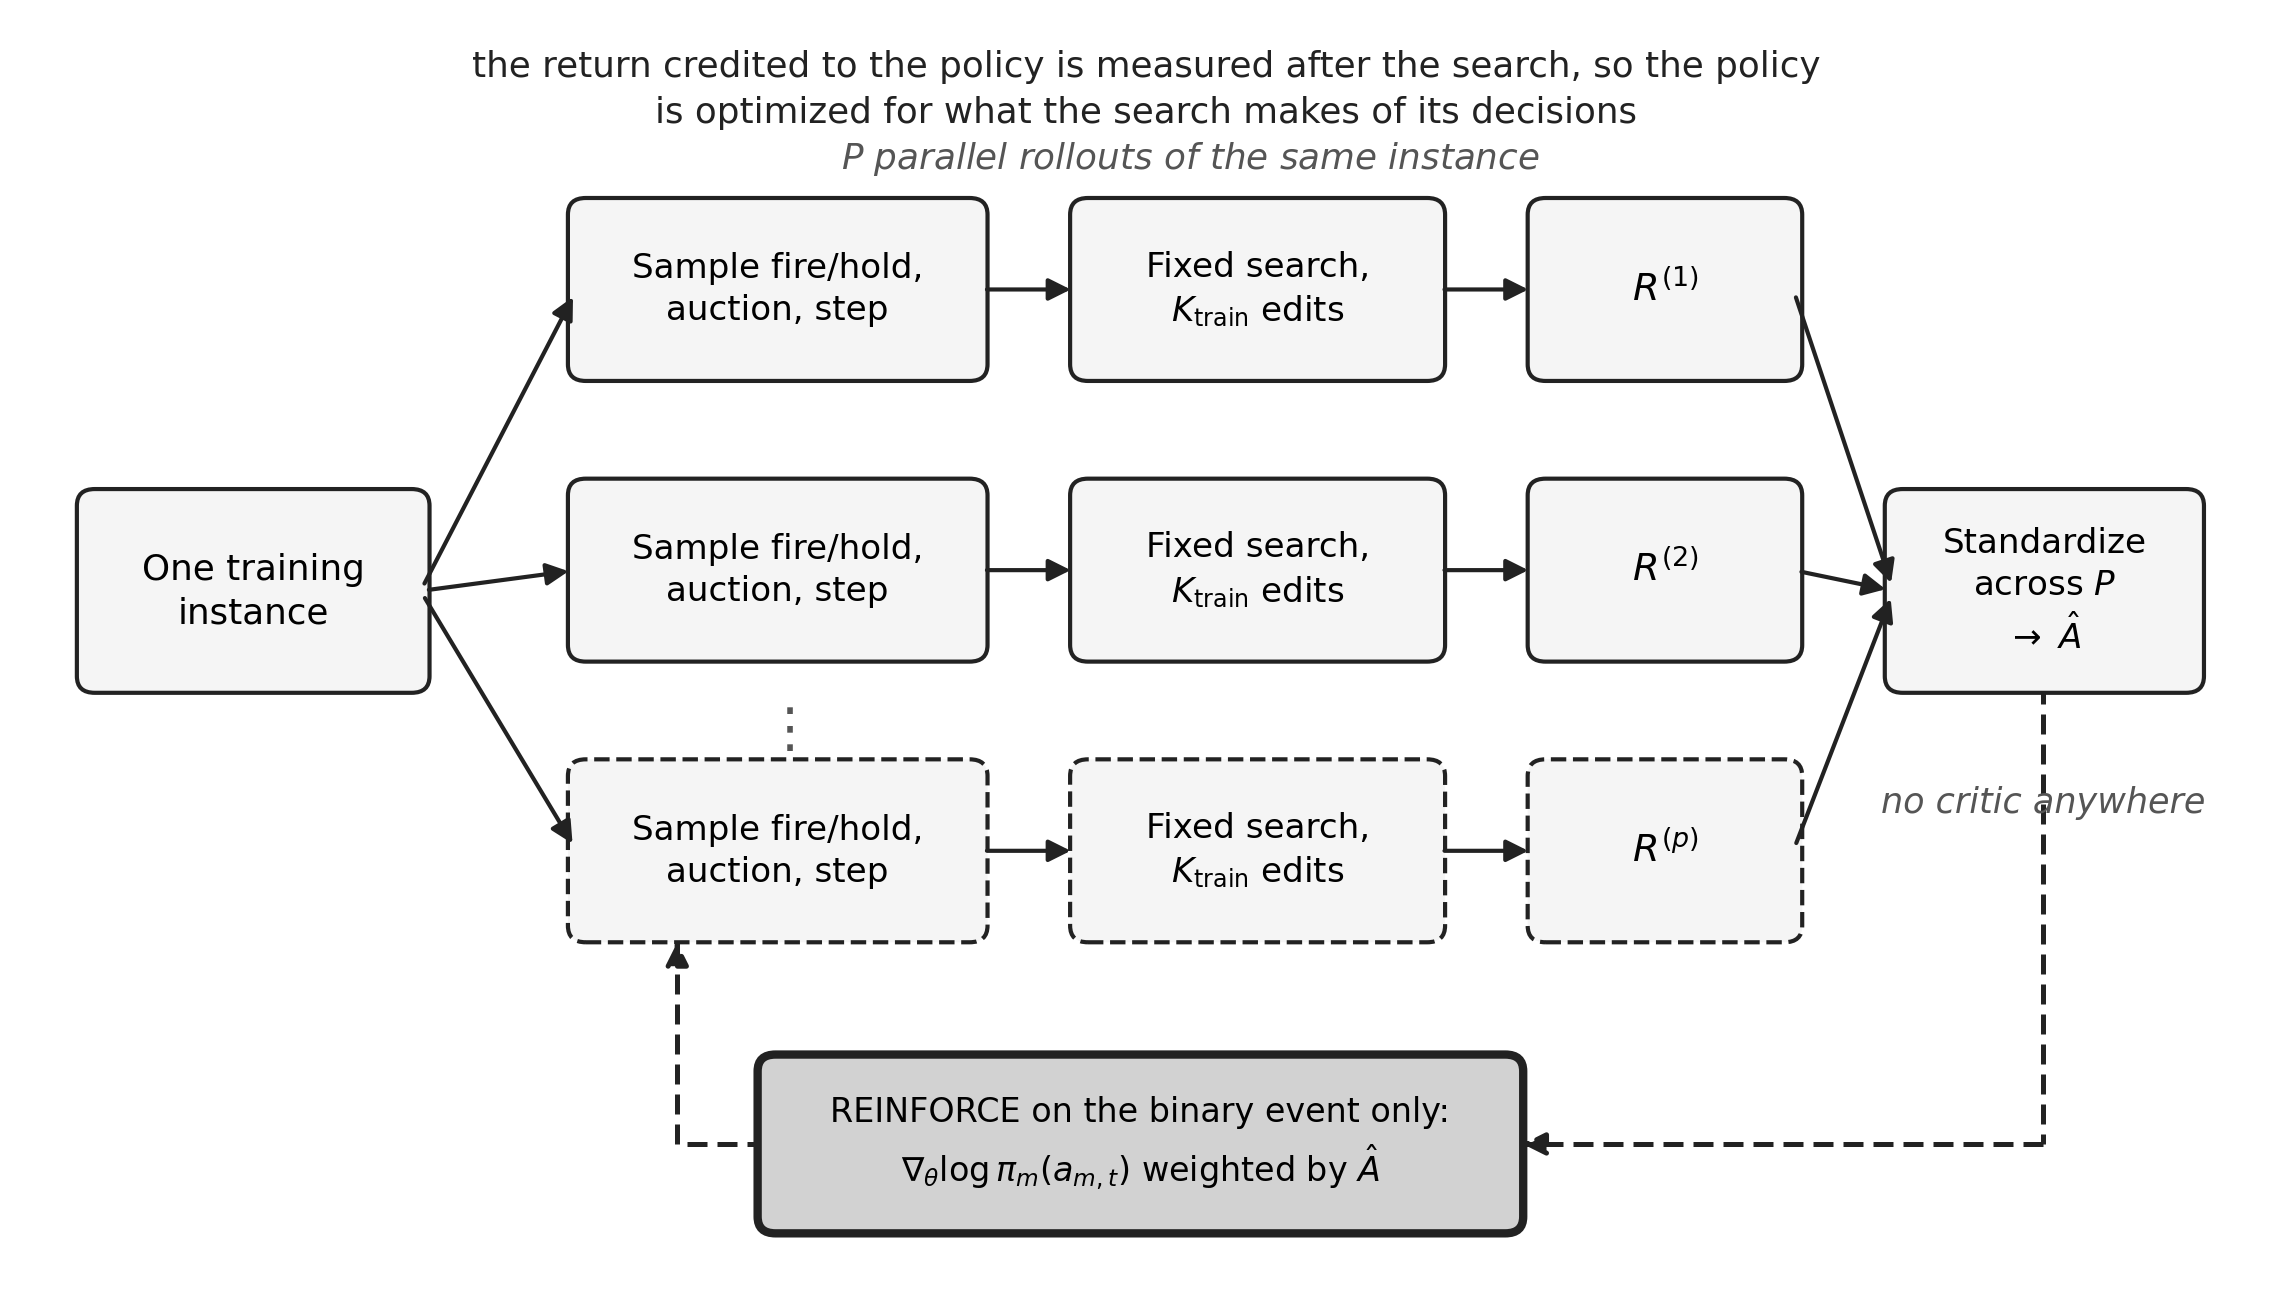
\includegraphics[width=\columnwidth]{figure/Training.png}
  \caption{Training. $P$ rollouts of one instance are sampled, each is passed
  through the fixed local search at a budget $K_{\mathrm{train}}$, and the
  post-search returns are standardized against one another to form the
  advantage. The gradient credits only the binary fire-or-hold event, not the
  target the assignment step chose. No value network appears at any point.}
  \label{fig:training}
\end{figure}

Two properties of this scheme are worth stating. First, the policy is
optimized for what the downstream machinery makes of its decisions rather than
for its own unsearched output, which is the relevant objective at deployment.
Second, because the search is fixed rather than learned, there is only one
moving target during training: the policy adapts to a stationary improvement
operator, rather than two networks each chasing the other's drift. The cost is
that the search absorbs some of the policy's mistakes before the objective is
measured, which attenuates the learning signal about exactly those mistakes;
Section~\ref{sec:limits} returns to this.

%% \section{Theoretical Analysis}
\label{sec:submodular}

This section establishes the two facts the decomposition rests on. Once the
firing weapons are fixed, assigning targets among them greedily by marginal
value attains at least half the stage optimum with no learned parameters
(Proposition~\ref{prop:auction-half}), and the guarantee holds for any firing
set, including one produced by all weapons deciding at the same instant. The
other half of the decision admits no such treatment: choosing which weapons
fire by what is best in the current stage can be arbitrarily far from optimal
(Proposition~\ref{prop:myopic-gap}). That gap is the entire job of the learned
policy.

Throughout we reuse the stage objective $f_t$ of Eq.~\eqref{eq:round-obj},
the firing set $F$, and the edge set $E_t$ introduced in
Section~\ref{sec:auction}, where $f_t$ was shown to be monotone
submodular~\cite{wang2013weapon} under a partition matroid induced by
Eq.~\eqref{eq:weapon_target_constraint}. Write
$\text{OPT}_t(F) = \max_{S_t \text{ feasible}} f_t(S_t)$ and
$\text{OPT}_t = \text{OPT}_t(\{1,\ldots,M\})$.

\subsection{Target Assignment Is Solved, Not Approximated}

%% ============================================================
%% COMMENTED OUT 2026-09-14: Propositions par-linear and seq-half.
%%
%% These two set up the standard case that simultaneous multi-agent decoding
%% needs a coordination mechanism, so that the assignment guarantee could then
%% be shown to remove the need for one. That argument turned out to be longer
%% than it needs to be: prop:auction-half holds for ANY firing set, which
%% already says the guarantee does not care whether the set was produced all
%% at once, and the comparison against sequential decoding is carried
%% empirically by Table~\ref{tab:main_results}.
%%
%% Restore if a reviewer asks why simultaneous decoding is safe in the
%% worst case rather than only on the benchmark. related_works.tex also
%% cited this pair; that sentence was rewritten when these were cut.
%% ============================================================
%% \begin{proposition}[Parallel decoding without an assignment mechanism: tight $\Theta(1/M)$]
%% \label{prop:par-linear}
%% Consider the idealized zero-communication parallel rule in which each weapon
%% $m$ simultaneously selects its own feasible pair of largest singleton value
%% $f_t(\{(m,n)\})$, with no visibility into the other weapons' same-stage
%% choices. Then $f_t(\mathrm{Par}_t) \geq \tfrac{1}{M}\text{OPT}_t$, and this
%% is tight.
%% \end{proposition}
%% \begin{proof}
%% \emph{Lower bound.} Let $e^\ast = \arg\max_{e\in E_t} f_t(\{e\})$. By
%% monotonicity and submodularity $f_t$ is subadditive, so for the optimal
%% feasible $S^\ast_t$ (with $|S^\ast_t|\leq M$),
%% $\text{OPT}_t \leq \sum_{e\in S^\ast_t} f_t(\{e\}) \leq M f_t(\{e^\ast\})$.
%% The weapon owning $e^\ast$ selects it, since $e^\ast$ is globally best and
%% hence best within its own part, so $f_t(\mathrm{Par}_t) \geq f_t(\{e^\ast\})
%% \geq \text{OPT}_t/M$.
%%
%% \emph{Tightness.} Take $M$ weapons and $M{+}1$ targets: a shared target $n_0$
%% of value $1$ and one private target per weapon of value $1-\varepsilon$, all
%% with $P\equiv 1$ and all pairs feasible. Every weapon's best singleton is
%% $n_0$, so $\mathrm{Par}_t$ sends all $M$ weapons to $n_0$, giving
%% $f_t(\mathrm{Par}_t)=1$, while assigning one weapon to $n_0$ and the rest to
%% their private targets gives $\text{OPT}_t = 1+(M{-}1)(1{-}\varepsilon)$. The
%% ratio tends to $1/M$ as $\varepsilon\to 0$.
%% \end{proof}
%%
%% \begin{proposition}[Sequential decoding carries a constant-factor guarantee]
%% \label{prop:seq-half}
%% An idealized sequential rule, in which each weapon in turn selects the
%% feasible pair of largest marginal gain given all pairs already selected this
%% stage, is the greedy algorithm for monotone submodular maximization under a
%% matroid constraint, and therefore guarantees
%% $f_t(\mathrm{Seq}_t) \geq \tfrac12\text{OPT}_t$~\cite{fisher1978analysis}.
%% \end{proposition}
%%
%% Propositions~\ref{prop:par-linear} and~\ref{prop:seq-half} are the standard
%% argument for why simultaneous multi-agent decoding needs a coordination
%% mechanism, and they are why the multi-agent reinforcement learning
%% literature has largely moved to sequential, auto-regressive action
%% generation: the multi-agent advantage decomposition
%% theorem~\cite{kuba2022trust} transforms the joint policy search into exactly
%% the sequential decision process of Proposition~\ref{prop:seq-half}, and it is
%% that sequencing which buys the monotonic improvement guarantees of
%% HATRPO/HAPPO~\cite{kuba2022trust} and MAT~\cite{wen2022mat}.
%%

Our pipeline does not coordinate the weapons' target choices better. It
removes the choice from them.

\begin{proposition}[Many-to-one marginal assignment is matroid greedy on the stage objective]
\label{prop:auction-half}
Fix stage $t$ and a firing set $F$, and let $\text{OPT}_t(F)$ be the maximum of $f_t$ over feasible allocations of the weapons in $F$. The many-to-one greedy assignment returns an allocation $S^{\text{gre}}_t$ with
\begin{equation}
f_t(S^{\text{auc}}_t) \;\geq\; \tfrac12\,\text{OPT}_t(F).
\end{equation}
\end{proposition}
\begin{proof}
First, the assignment score equals the exact marginal gain of $f_t$. Let $S$ be the allocation so far and $S_{n'}$ the weapons already assigned to target $n'$. Adding $(m',n')$ changes only the $n'$ summand of Eq.~\eqref{eq:round-obj}:
\begin{align*}
f_t(S \cup \{(m',n')\}) - f_t(S)
&= V_{n'}\rho_{n'}^{(t)}\Big[\textstyle\prod_{m \in S_{n'}}(1-P_{m,n'}) \\
&\qquad\qquad - \textstyle\prod_{m \in S_{n'} \cup \{m'\}}(1-P_{m,n'})\Big] \\
&= V_{n'}\rho_{n'}^{(t)} \Big(\textstyle\prod_{m \in S_{n'}}(1-P_{m,n'})\Big)\big[1-(1-P_{m',n'})\big] \\
&= V_{n'}\rho_{n'}^{(t)}\,\sigma_{n'}\,P_{m',n'} \;=\; b_{m',n'},
\end{align*}
which is the quantity of Eq.~\eqref{eq:marginal-bid}. Second, the rule is greedy in that quantity: each iteration takes the single largest score over all unassigned weapons and legal targets, and never revokes an assignment. It is therefore the greedy algorithm for maximizing the monotone submodular $f_t$ under the partition matroid constraint, which attains at least $\tfrac12$ of the constrained optimum~\cite{fisher1978analysis}.
\end{proof}

The factor $\tfrac12$ is a worst-case floor that holds regardless of the scale of the problem: it does not degrade as the number of weapons $M$ grows. It is also close to the best attainable, since no polynomial-time method can guarantee more than $1-1/e$ for this problem class~\cite{feige1998threshold}, and the alternatives analyzed in Section~\ref{sec:submodular} carry either no guarantee or one that decays as $1/M$. The floor is also loose in practice. On the $(5,5,5)$ and $(5,7,5)$ benchmark configurations, where $\text{OPT}_t(F)$ can be computed exactly by enumerating every feasible allocation of the firing weapons, the rule attains a mean 99.3\% of the stage optimum over 77 policy-generated stages (ten instances per configuration, distribution of Section~\ref{sec:data}) and never falls below 87.1\%. The $\tfrac12$ bound is thus a guarantee against adversarial instances, not a description of typical behavior.
%% Measured 2026-08-24 by code_DWTA/eval_auction_stage_ratio.py (result/auction_stage_ratio.txt):
%% (5,5,5) mean 0.9939 min 0.8711 over 38 stages; (5,7,5) 0.9918/0.8782 over 39; combined 77 stages
%% mean 0.9928 min 0.8711. A third probe config (5,15,5) gave 0.9973/0.9496 (43 stages) -- not reported
%% in prose per author decision (non-benchmark config). Ratio = f_t(auction)/OPT_t(F) with F fixed to
%% the trained SCoPE-Comm policy's firing set, OPT by exhaustive enumeration. Stages with empty F or
%% no legal target excluded.

What matters for the rest of the argument is the quantifier in
Proposition~\ref{prop:auction-half}, not the constant.

\begin{remark}
\label{rem:auction-kills-pileon}
Proposition~\ref{prop:auction-half} holds for \emph{any} firing set, in
particular one produced by $M$ weapons deciding simultaneously and
independently. Weapons deciding at the same instant would normally contend
for the same target, and a communication layer or conflict handler exists to
settle that contention. Here there is nothing to settle: no weapon chooses a
target, so the choices that would collide are never made. The guarantee is
obtained at one network call per stage rather than $M$.
\end{remark}

\subsection{Participation Cannot Be Decided Per Stage}

Proposition~\ref{prop:auction-half} is conditional on $F$. It says nothing
about how $F$ should be chosen, and the natural per-stage answer is to fire
every weapon whose best available marginal value is positive. That answer is
unboundedly bad.

\begin{proposition}[Myopic participation is arbitrarily suboptimal]
\label{prop:myopic-gap}
Let $\textsc{Myopic}$ be the rule that, at every stage, fires every weapon
with at least one legal target of positive marginal value, and assigns
targets by greedy marginal assignment. For every $\kappa > 0$ there is a DWTA instance on
which the value destroyed by $\textsc{Myopic}$ is less than $\kappa$ times
the value destroyed by an optimal policy. No constant-factor guarantee for
$\textsc{Myopic}$ exists.
\end{proposition}
\begin{proof}
Take $T=2$, $M=1$, $N=2$. The single weapon has ammunition $A_1 = 1$, with
$P_{1,1}=P_{1,2}=p \in (0,1]$. Target 1
has value $V_1 = 1$ and time window $TW_1 = \{1\}$; target 2 has value
$V_2 = V > 0$ and time window $TW_2 = \{2\}$.

At stage 1 the only legal engagement is target 1, whose marginal value
$V_1 p = p$ is positive, so $\textsc{Myopic}$ fires and exhausts the
weapon's ammunition. At stage 2 target 2 is legal but the weapon has no
ammunition, so nothing is engaged. $\textsc{Myopic}$ destroys $p$.

The policy that holds at stage 1 and fires at target 2 at stage 2 is
feasible and destroys $pV$. Hence the optimum destroys at least $pV$, and
the ratio is at most $p/(pV) = 1/V$. Choosing $V > 1/\kappa$ gives the
claim.
\end{proof}

\begin{remark}
\label{rem:myopic-is-the-job}
The instance in Proposition~\ref{prop:myopic-gap} isolates the one quantity
no within-stage mechanism can access: the value of \emph{not} acting, which
is zero within the stage and realized only later. Both the assignment
guarantee (Proposition~\ref{prop:auction-half}) is per-stage, and so says
nothing about it. This is the precise sense in which the
decomposition of Section~\ref{sec:method} assigns learning only the part
that cannot be obtained otherwise. It is also directly measurable: the
Greedy baseline of Table~\ref{tab:main_results} is $\textsc{Myopic}$: it uses
the same assignment rule as our pipeline and fires every weapon it can, so
the margin between it and the learned pipeline is an empirical estimate of
how much this gap costs on realistic instances rather than adversarial ones.
\end{remark}

\begin{remark}
\label{rem:gap-interpretation}
Proposition~\ref{prop:auction-half} concerns an idealized rule, not a
trained network, and bounds a single stage rather than a full $T$-stage
trajectory. Value missed at one stage is not necessarily
lost: it remains on the battlefield, is re-observed through the updated
$\rho_n^{(t+1)}$, and can be recovered later, which is one reason measured
gaps are far smaller than the worst cases above. Proposition~\ref{prop:myopic-gap}
is the exception, and deliberately so: its construction uses a closing time
window precisely so that the missed value cannot be recovered, which is what
makes the participation decision genuinely multi-stage rather than merely
harder-to-see.
\end{remark}
  %% retired 2026-09-14: the two
%% propositions now sit in method.tex beside the steps they justify.
\section{Experimental Results}
\label{sec:results}

\subsection{Experimental Setup}
\label{sec:data}

All experiments are conducted on a machine equipped with an NVIDIA GeForce RTX 5080 GPU (16\,GB) and an AMD Ryzen 9 9900X 12-core CPU (32\,GB), running Windows 11. The model is implemented in Python 3.12 with PyTorch and CUDA 12.8. Training requires approximately two hours per seed over 400 training steps.

Training instances are generated following the parameter distribution shown in Table~\ref{tab:parameter_distributions}. The policy is trained on instances with $M, N, T \in [5,7]$, drawn at random each episode from this distribution.

Instances are partitioned into three disjoint sets: a training set (generated online from the same distribution at each episode), a validation set (separate instances of the same size range, evaluated every ten epochs under greedy decoding for model selection), and a test set of ten independent benchmark replications per configuration (120 instances total). The twelve test configurations, ranging from $(5,5,5)$ to $(70,100,15)$ and shown in Table~\ref{tab:problem_instance_scales}, span four size tiers (Small, Medium, Large, Battlefield) and are never seen during training. Configurations are restricted to $N \geq M$ (targets at least as numerous as weapons), reflecting resource-constrained defense scenarios.

\begin{table}[htbp]
\centering
\small
\caption{Instance parameter distribution. $\mathcal{Z}(a,b)$ denotes discrete uniform on $\{a, \ldots, b\}$. $D_m$ is the number of stages before a weapon can fire again; $D_m=1$ permits every-stage firing.}
\label{tab:parameter_distributions}
\begin{tabular}{l|l}
\hline
\textbf{Attribute} & \textbf{Distribution} \\ \hline
Target Value $V_n$ & $U(1, 10)$ \\
Reload Time $D_m$ & $\mathcal{Z}(1, 2)$ \\
Ammunition $A_m$ & $\mathcal{Z}(1, \lfloor T/2\rfloor{+}1)$ \\
Start Time $t_{n,\text{start}}$ & $\mathcal{Z}(0, T{-}1)$ \\
End Time $t_{n,\text{end}}$ & $T{-}1$ \\
Damage Rate $P$ & $U(0.3, 0.9)$ \\ \hline
\end{tabular}
\end{table}

\begin{table}[htbp]
\centering
\small
\caption{Test problem configurations. Each configuration uses ten fixed, seed-controlled instances identical across all methods.}
\label{tab:problem_instance_scales}
\begin{tabular}{c|c|c}
\hline
\textbf{Tier} & \textbf{(M,N,T)} & \textbf{Instances} \\ \hline
\multirow{3}{*}{Small}      & (5,5,5)    & 10 \\
                            & (5,7,5)    & 10 \\
                            & (10,15,5)  & 10 \\ \hline
\multirow{3}{*}{Medium}     & (15,15,5)  & 10 \\
                            & (15,20,5)  & 10 \\
                            & (20,30,5)  & 10 \\ \hline
\multirow{3}{*}{Large}      & (30,30,10) & 10 \\
                            & (30,40,10) & 10 \\
                            & (40,50,10) & 10 \\ \hline
\multirow{3}{*}{Battlefield} & (50,50,15) & 10 \\
                            & (50,70,15) & 10 \\
                            & (70,100,15) & 10 \\ \hline
\end{tabular}
\end{table}

%% RESOLVED 2026-08-23: Table~\ref{tab:problem_instance_scales} now states 10 instances/config,
%% matching what every reported run actually used (seed-controlled, fixed across methods).
%% 2026-09-14: distribution table now matches generate_moderate_temporal_instance
%% (V = U(2,6) + U(2,5)*t_start/(T-1), ammo Z(1,floor(T/2)+1), P ~ U(0.3,0.9)).
%% Reload is reported as the firing cadence D_m = prep + 1, so code prep in {0,1}
%% is tabulated as Z(1,2); see DWTA_Simulator.py:317.


Model and training hyperparameters follow standard practice in GNN-based
combinatorial optimization, detailed in Table~\ref{tab:hyperparameters}. No
systematic tuning was performed except on the search budget $K$
(Section~\ref{sec:budget}), whose impact is studied directly. Other configurations may yield better results.

\begin{table}[h]
\centering
\small
\caption{Selected model and training hyperparameters.}
\label{tab:hyperparameters}
\begin{tabular}{ll}
\hline
\textbf{Parameter} & \textbf{Value} \\ \hline
Message-passing layers $L$ & 3 \\
Hidden/embedding dimension $H$ & 128 \\
Attention heads (ablation only, Eq.~\eqref{eq:comm-attn}) & 8 \\
Dropout (residual blocks) & 0.1 \\
Optimizer & Adam \\
Learning rate & $5 \times 10^{-4}$ (cosine decay to $1\%$) \\
Weight decay & $1 \times 10^{-2}$ \\
Gradient-norm clip & 1.0 \\
Instances per training step & 15 \\
Parallel rollouts per instance $P$ & 10 \\
Ammunition bonus $\lambda_{\text{ammo}}$ (Eq.~\eqref{eq:return}) & 0.1 \\
Search budget in training $K_{\text{train}}$ & 3 \\
Search budget at evaluation $K$ & 10 (Table~\ref{tab:budget}) \\ \hline
\end{tabular}
\end{table}

%% Values above verified against common/Dynamic_HYPER_PARAMETER.py and common/DWTA_GNN_comm_sinkhorn.py
%% on 2026-08-23 (EMBEDDING_DIM=128, HEAD_NUM=8, ACTOR_LEARNING_RATE=5e-4, ACTOR_WEIGHT_DECAY=1e-2,
%% ResidualBlock/MultiheadAttention dropout=0.1, Adam). Training-loop values re-verified
%% 2026-09-12 against rl/DWTA_GNN_TRAIN_search_in_loop.py (k_edits=3, k_eval=10, batch 15,
%% para 10, ammo_coef=0.1).
%%
%% RESOLVED 2026-08-23: sinkhorn_scale ablation run (eval_sinkhorn_ablation.py, result/sinkhorn_ablation.txt):
%% scale as trained (0.0213) vs forced to 0, all 12 configs, same instances -- mean 0.1528 vs 0.1527,
%% per-config deltas within +-0.0024 (both signs, noise). Term is INACTIVE; disclosed in one sentence
%% at the end of Section~\ref{sec:comm}.


\subsubsection{Baseline Methods}

We compare against three families of baselines: an exact solver, two
non-learned heuristics, and three learned construction policies.

\paragraph{Exact} The DWTA formulation of Section~\ref{sec:problem} is a
mixed-integer nonlinear program, which we solve with
SCIP~\cite{bestuzheva2023scip} under a 600\,s time limit per instance. When
optimality is not proven within that budget, SCIP reports its best incumbent.

\paragraph{Heuristics} \textsc{Greedy} assigns, at every stage, the
weapon-target pair with the largest immediate marginal destroyed value,
updates that target's remaining value, and repeats until no legal pair
remains. This is the assignment rule of Section~\ref{sec:auction} applied to
every weapon that can fire, which makes it exactly the $\textsc{Myopic}$ rule
of Proposition~\ref{prop:myopic-gap}. It is the baseline that isolates what
the learned fire-or-hold decision contributes: it and our method assign
targets identically and differ only in which weapons fire.
\textsc{Auction} instead matches weapons to targets by the price mechanism of
Bertsekas~\cite{bertsekas1988auction}. Targets carry prices that rise as
weapons bid on them, an incumbent is displaced when outbid, and a weapon
holds fire when no target's remaining value exceeds its price. Prices admit
one weapon per target, so this baseline cannot concentrate several weapons on
a single target.

\paragraph{Learned construction policies} All three build a schedule
autoregressively, one decision at a time, re-observing the state after each.
They differ in how a decision is parameterized and in what the encoder sees.

\textsc{Sequential} decodes one assignment at a time. At
every step it forms a single softmax over all $M \times N$ weapon-target edges
plus one global no-op, samples one edge, applies it, and re-runs the full
edge-aware GNN encoder on the updated state. It therefore chooses \emph{which
weapon acts} and \emph{which target it engages} jointly at each step, and the
kill probability $P_{mn}$ enters the encoder directly as an edge feature.

AM~\cite{kool2018attention} is the attention model of Kool et al., run
unmodified through RL4CO~\cite{berto2023rl4co}. Its encoder is a Transformer
over target nodes, evaluated once per instance; the decoder then attends to
those fixed embeddings through a context query. Because target values change
as damage accumulates, the static-embedding default is unsound here, so
remaining value is supplied to the decoder as an explicit dynamic embedding.
The decision order is fixed in advance, round-major and weapon-minor, so the
step index prescribes which weapon acts and the pointer selects only its
target or a no-op.

POMO~\cite{kwon2020pomo} shares AM's architecture and differs in its rollout
scheme: several trajectories are drawn per instance from forced-distinct
starting actions, and their mean serves as the REINFORCE baseline. We report
POMO under single-path greedy decoding rather than best-of-multistart, so that
its inference budget matches every other method in the table.

All three learned baselines are trained on the same curriculum under the same
optimizer settings, and all neural methods are evaluated zero-shot at every
tier with no fine-tuning on the test configurations.

\subsection{Main Results}
\label{sec:main-results}

Methods are compared on the normalized remaining value, the fraction of the
initial target value still standing when the engagement ends, for which lower
is better.
%% Generated by code_DWTA/eval_final_table.py from the three fire/hold-only
%% checkpoints (seeds 5, 6, 7), result/final_table_nocomm.txt. (NOT
%% final_table_multiseed.txt, which is the older with-communication run and
%% has mean 0.1197 at K=10 rather than the reported 0.1179.)
%% Baseline columns are carried over from the previous benchmark run: verified
%% comparable because both use the same generator, seed 123, and the same ten
%% instances per configuration -- the Sequential mean reproduces to 0.1432 in
%% both, to four decimals.

\begin{table*}[t]
\centering
\scriptsize
\caption{Main results across twelve held-out test configurations.
Normalized remaining value (lower is better). Our column reports the mean over three seeds followed by the across-seed standard deviation. Every method constructs its schedule in a single pass, so the comparison is at matched inference effort; what the local search adds on top is reported separately in Section~\ref{sec:budget}. SCIP uses a 600\,s limit and reports its incumbent; at the two largest configurations it fails to find a competitive solution. Bold marks the best method per configuration.}
\label{tab:main_results}
\begin{tabular}{@{}llcccccccc@{}}
\toprule
Tier & Config & SCIP & Greedy & Auction & AM & POMO & Sequential & Ours \\
\midrule
\multirow{3}{*}{Small}
 & (5,5,5)     & \textbf{0.148} & 0.598 & 0.362 & 0.249 & 0.243 & 0.169 & 0.190 $\pm$ .000 \\
 & (5,7,5)     & \textbf{0.199} & 0.623 & 0.455 & 0.446 & 0.447 & 0.307 & 0.245 $\pm$ .000 \\
 & (10,15,5)   & \textbf{0.192} & 0.619 & 0.418 & 0.446 & 0.488 & 0.300 & 0.225 $\pm$ .001 \\
\midrule
\multirow{3}{*}{Medium}
 & (15,15,5)   & \textbf{0.087} & 0.533 & 0.266 & 0.288 & 0.315 & 0.096 & 0.094 $\pm$ .000 \\
 & (15,20,5)   & \textbf{0.138} & 0.616 & 0.363 & 0.480 & 0.508 & 0.207 & 0.166 $\pm$ .000 \\
 & (20,30,5)   & \textbf{0.176} & 0.638 & 0.448 & 0.548 & 0.584 & 0.295 & 0.209 $\pm$ .000 \\
\midrule
\multirow{3}{*}{Large}
 & (30,30,10)  & 0.015 & 0.355 & 0.078 & 0.164 & 0.093 & 0.016 & \textbf{0.012} $\pm$ .001 \\
 & (30,40,10)  & 0.045 & 0.407 & 0.177 & 0.256 & 0.136 & \textbf{0.032} & 0.037 $\pm$ .002 \\
 & (40,50,10)  & 0.051 & 0.331 & 0.150 & 0.261 & 0.144 & \textbf{0.028} & 0.028 $\pm$ .001 \\
\midrule
\multirow{3}{*}{Battlefield}
 & (50,50,15)  & 0.157 & 0.361 & 0.156 & 0.195 & \textbf{0.077} & 0.088 & 0.084 $\pm$ .002 \\
 & (50,70,15)  & 0.992 & 0.390 & 0.171 & 0.268 & 0.099 & 0.080 & \textbf{0.077} $\pm$ .002 \\
 & (70,100,15) & 0.993 & 0.403 & 0.177 & 0.306 & 0.106 & 0.100 & \textbf{0.096} $\pm$ .001 \\
\midrule
 & \textbf{Mean} & 0.266 & 0.490 & 0.268 & 0.326 & 0.270 & 0.143 & \textbf{0.122} \\
\bottomrule
\end{tabular}
\end{table*}

At matched inference effort, the mean objective across the twelve
configurations is 0.122, against 0.143 for the strongest neural baseline
(Sequential), a 14.9\% relative reduction. Every non-exact baseline is beaten
on the mean.

The table answers two questions at once, and they are the two the
decomposition rests on. \textsc{AM}, \textsc{POMO} and \textsc{Sequential}
all learn the target choice as well as the firing decision, and all three are
beaten: 0.326, 0.270 and 0.143 against our 0.122. Removing target selection
from the policy therefore costs nothing that a learned target head was
supplying. \textsc{Greedy}, at the other end, assigns targets by the same rule
we do and differs only in that no policy decides which weapons fire; it scores
0.490. The firing decision is thus where essentially all of the value sits,
and it is the one part for which Proposition~\ref{prop:myopic-gap} rules out
any per-stage substitute. Learning less does not cost accuracy here; learning
the right part is what buys it.

The per-configuration picture is more informative than the mean, and splits
cleanly by tier. Against SCIP, we lose all six Small and Medium
configurations and win all six Large and Battlefield ones. That is the
expected pattern: at small scale the solver still proves or nearly proves
optimality within its budget, and no heuristic should beat it there; at large
scale its branch-and-bound no longer reaches a competitive incumbent, failing
outright at the two largest configurations. Against Sequential, the
strongest learned baseline, we win 9 of 12 and tie at (40,50,10),
losing only (5,5,5) by 0.021 and (30,40,10) by 0.005. Against all learned
baselines together we are best at 8 of 12; the remaining loss is (50,50,15),
where POMO reaches 0.077 against our 0.084.

All results are reported over three seeds. Across-seed standard deviations
are between 0.000 and 0.002, smaller than the gap to the nearest competing
method at every configuration, so the ordering of methods does not depend on
which training run is used.

%% Measured by code_DWTA/measure_method_timing.py (Greedy, Auction, Sequential,
%% ours) and code_DWTA/measure_rl4co_timing.py (AM, POMO), both on the same ten
%% seed-123 instances per configuration. CUDA-synchronized, warm-up passes
%% discarded, one instance at a time: RL4CO would batch all ten into a single
%% forward, which would credit AM and POMO with parallelism no other method is
%% given. Raw output in result/timing_methods.txt and result/timing_rl4co.txt.

\begin{table}[t]
\centering
\small
\caption{Mean wall-clock time per instance in seconds, averaged over the three
configurations in each tier. Every column is the cost of producing one
schedule: encoding, every network call, the assignment step, and all
environment simulation, measured end to end with CUDA synchronization after
untimed warm-up passes. Our column is the construction pass alone, at
$K{=}0$, which is the budget the table's objectives are reported at; what the
local search adds on top is in Section~\ref{sec:budget}. All methods decode
one instance at a time, since RL4CO would otherwise batch AM and POMO into a
single forward and credit them with parallelism no other method is given.
SCIP is omitted: it is given a fixed 600\,s budget per instance rather than
run to completion, so its time is a setting rather than a measurement
(Appendix~\ref{app:scip}).}
\label{tab:timing}
\begin{tabular}{@{}lcccccc@{}}
\toprule
Tier & Greedy & Auction & AM & POMO & Sequential & Ours \\
\midrule
Small       & \textbf{0.029} & 0.113 & 0.075 & 0.093 & 0.055 & 0.032 \\
Medium      & \textbf{0.053} & 0.159 & 0.153 & 0.153 & 0.122 & 0.063 \\
Large       & \textbf{0.184} & 0.558 & 0.651 & 0.603 & 0.497 & 0.203 \\
Battlefield & \textbf{0.527} & 1.562 & 1.618 & 1.604 & 1.315 & 0.577 \\
\midrule
\textbf{Mean} & \textbf{0.199} & 0.598 & 0.625 & 0.613 & 0.497 & 0.218 \\
\bottomrule
\end{tabular}
\end{table}

Table~\ref{tab:timing} reports what each method costs to run. Our pipeline is
the fastest of every method that learns anything, at 0.218\,s per instance
against 0.497\,s for the sequential decoder and roughly 0.62\,s for AM and
POMO, and the margin widens with scale: at the Battlefield tier it is 0.577\,s
against 1.315\,s. The reason is structural. Construction calls the network
once per stage and decides all $M$ weapons in that one call, whereas a
sequential decoder calls it once per weapon per stage, so its cost grows with
the size of the force while ours does not. Only \textsc{Greedy} is faster, at
0.199\,s, and it has no network to run at all.

Taken together with the objective, this is the result the paper rests on. The
one method that beats us on time is the worst in the table on quality, at
0.490 against our 0.122. The methods that come closest on quality are two to
six times slower. Against \textsc{Sequential}, the strongest learned baseline,
we are better on the objective at nine of twelve configurations and
2.3 times faster on average, so the comparison does not trade one against the
other.

\subsection{Inference-Time Improvement}
\label{sec:budget}

Once a schedule has been constructed it can still be improved without
touching the model. The search flips one fire-or-hold decision, re-simulates
the episode under the same assignment rule, and keeps the change only if the
objective improves, repeating this up to $K$ times
(Section~\ref{sec:local-search}). Nothing is learned here: the budget $K$ buys
computation at inference, not parameters.

Because a flip is kept only on strict improvement, the objective is
non-increasing in $K$, so the informative question is not whether the curve
descends but where it stops. Table~\ref{tab:budget} reports the sweep and, for
each configuration, the mean index of the last accepted flip within a $K{=}30$
probe.

\begin{table}[t]
\centering
\small
\caption{Edit-budget sweep, mean over three seeds. \emph{last accept} is the
mean index of the final accepted flip within a $K{=}30$ probe; a value near 30
indicates the search was still finding improvements when the budget ran out.}
\label{tab:budget}
\begin{tabular}{@{}lccccc@{}}
\toprule
Config & $K{=}0$ & $K{=}3$ & $K{=}10$ & $K{=}30$ & last accept \\
\midrule
(5,5,5)     & 0.1901 & 0.1825 & 0.1740 & 0.1660 & 11.5 \\
(5,7,5)     & 0.2451 & 0.2381 & 0.2347 & 0.2341 & 7.0 \\
(10,15,5)   & 0.2248 & 0.2240 & 0.2212 & 0.2167 & 13.3 \\
(15,15,5)   & 0.0940 & 0.0925 & 0.0918 & 0.0905 & 12.9 \\
(15,20,5)   & 0.1661 & 0.1647 & 0.1597 & 0.1550 & 19.8 \\
(20,30,5)   & 0.2086 & 0.2070 & 0.2040 & 0.1985 & 17.7 \\
(30,30,10)  & 0.0121 & 0.0118 & 0.0113 & 0.0105 & 21.3 \\
(30,40,10)  & 0.0373 & 0.0366 & 0.0355 & 0.0336 & 21.8 \\
(40,50,10)  & 0.0279 & 0.0275 & 0.0263 & 0.0248 & 19.4 \\
(50,50,15)  & 0.0839 & 0.0838 & 0.0837 & 0.0837 & 21.2 \\
(50,70,15)  & 0.0771 & 0.0770 & 0.0769 & 0.0767 & 20.6 \\
(70,100,15) & 0.0960 & 0.0959 & 0.0958 & 0.0956 & 21.7 \\
\midrule
\textbf{Mean} & 0.1219 & 0.1201 & 0.1179 & \textbf{0.1155} & 17.4 \\
\bottomrule
\end{tabular}
\end{table}

Two patterns matter. The gain is modest in absolute terms, 0.1219 to 0.1155,
a 5.2\% relative reduction across the full budget, because the construction
policy is now trained against the searched objective and therefore already
produces schedules the search has little left to fix. That is the intended
behaviour of training through the search, not a weakness of the search.

Second, where the curve flattens scales with problem size. At (5,7,5) the last
accepted flip is at index 7 on average, and the $K{=}10$ and $K{=}30$ columns
differ by 0.001. At the Large and Battlefield configurations the last accepted
flip sits around 20, so the search is still finding improvements when a budget
of 30 expires. A larger schedule offers more slots worth editing, and
because quality never falls as $K$ grows, an operator can
spend accordingly: a tight decision cycle stops at $K{=}3$ and banks most of
the gain, a loose one keeps going.

%% ============================================================
%% COMMENTED OUT 2026-09-14.
%% This section compared two sources of the fire/hold decision: our parallel
%% policy, and the Sequential decoder with its target choices discarded. That
%% second arm is not a clean control. Sequential decides firing and targeting
%% in one step, choosing an edge because a particular target is attractive, so
%% stripping the target away removes the reason the weapon was selected at all.
%% The honest version of this comparison would decide fire/hold weapon by
%% weapon and then assign, against deciding all at once and then assigning,
%% with the same policy in both arms; that needs a separately trained
%% sequential participation policy, since ours is trained to see all weapons
%% at once.
%%
%% It is also redundant. Proposition~\ref{prop:auction-half} holds for ANY
%% firing set, so the guarantee does not care whether the set was produced
%% simultaneously, and Table~\ref{tab:main_results} already shows the parallel
%% pipeline beating the Sequential decoder outright. Restore only if a
%% reviewer asks for the direct comparison AND the sequential participation
%% policy is trained.
%% ============================================================
%% \subsection{Which Decision Needs Learning}
%% \label{sec:firehold-source}
%%
%% Proposition~\ref{prop:auction-half} holds for any firing set, so the source of
%% that set should matter less than its quality. We test this by fixing the
%% pipeline, keeping the same assignment rule, revision, instances and budget, and
%% changing only where the fire/hold decision comes from. The sequential arm runs
%% the sequential decoder to completion on a copy of the live state and keeps only
%% which weapons fired, discarding its target choices exactly as the parallel
%% policy's are discarded.
%%
%% \begin{table}[t]
%% \centering
%% \small
%% \caption{Source of the fire/hold decision, everything else fixed. Normalized
%% remaining value, lower is better. \emph{Seq.\ alone} uses the sequential
%% decoder's own target choices, with no assignment step and no revision.}
%% \label{tab:firehold-source}
%% \begin{tabular}{@{}lcccccc@{}}
%% \toprule
%% & & \multicolumn{2}{c}{parallel} & \multicolumn{2}{c}{sequential} \\
%% \cmidrule(lr){3-4}\cmidrule(lr){5-6}
%% Config & Seq.\ alone & $K{=}0$ & $K{=}10$ & $K{=}0$ & $K{=}10$ \\
%% \midrule
%% (5,5,5)     & 0.1694 & 0.2486 & 0.1794 & 0.1736 & 0.1605 \\
%% (5,7,5)     & 0.3071 & 0.3213 & 0.2696 & 0.3093 & 0.2868 \\
%% (10,15,5)   & 0.2996 & 0.2911 & 0.2640 & 0.3011 & 0.2891 \\
%% (15,15,5)   & 0.0958 & 0.1215 & 0.1108 & 0.1003 & 0.0984 \\
%% (15,20,5)   & 0.2073 & 0.2150 & 0.1831 & 0.2154 & 0.1950 \\
%% (20,30,5)   & 0.2953 & 0.2599 & 0.2302 & 0.3076 & 0.2857 \\
%% (30,30,10)  & 0.0162 & 0.0153 & 0.0122 & 0.0153 & 0.0134 \\
%% (30,40,10)  & 0.0317 & 0.0361 & 0.0331 & 0.0344 & 0.0304 \\
%% (40,50,10)  & 0.0283 & 0.0298 & 0.0287 & 0.0299 & 0.0267 \\
%% (50,50,15)  & 0.0878 & 0.0972 & 0.0917 & 0.0852 & 0.0849 \\
%% (50,70,15)  & 0.0798 & 0.0869 & 0.0811 & 0.0783 & 0.0778 \\
%% (70,100,15) & 0.1003 & 0.1103 & 0.1063 & 0.0992 & 0.0988 \\
%% \midrule
%% \textbf{Mean} & 0.1432 & 0.1528 & \textbf{0.1325} & 0.1458 & 0.1373 \\
%% \bottomrule
%% \end{tabular}
%% \end{table}
%%
%% Unrevised, the sequential source is better (0.1458 vs 0.1528), as
%% Propositions~\ref{prop:par-linear} and~\ref{prop:seq-half} predict. The
%% ordering reverses at $K{=}10$: 0.1325 against 0.1373. Both beat the sequential
%% decoder using its own targets (0.1432), so delegating assignment costs nothing.
%%
%% The reversal is not evidence that simultaneous decisions are better; the
%% $K{=}0$ columns say otherwise. It is that parallel-produced schedules are more
%% improvable at equal budget. The sequential source still wins 7 of 12
%% configurations, so the mean is carried by margin, not by uniform superiority, most visibly at (20,30,5), 0.2302 against 0.2857.
%%
%% One caveat weakens the sequential arm: the revision policy used here was
%% trained on parallel-produced schedules, so the sequential arm is
%% off-distribution. The parallel win is conservative; the sequential numbers are
%% a lower bound.
%%

\subsection{Ablation Studies}
\label{sec:ablation}

Each of the following measures something the framework could have contained
and does not. Multi-agent construction policies normally give agents a way to
see one another before they commit, through a communication layer or a
conflict handler, because agents deciding at the same instant will otherwise
contend for the same resource. Ours has neither. The contended resource here
is the target, no weapon in this pipeline chooses one, and the assignment step
allocates targets after participation is already fixed, so there is nothing
left for the weapons to coordinate over. The same question arises for the
revision step, which could plausibly learn where to edit rather than propose
uniformly at random. In each case we built the richer variant, trained it
under an identical recipe, and kept the smaller one only where the measurement
said the addition did not earn its place.


\subsubsection{Weapon-to-Weapon Communication}
\label{sec:comm-ablation}

Remark~\ref{rem:auction-kills-pileon} predicts that inter-agent communication
should buy nothing here, because the contention it exists to resolve is over
targets and no weapon in this pipeline chooses one. We tested that prediction
by adding one multi-head self-attention layer over the $M$ weapon embeddings,
placed between the encoder and the scoring heads,
\begin{equation}
\label{eq:comm-attn}
\bm{C} = \text{MHA}\!\left(\bm{H}^{\text{wpn}}, \bm{H}^{\text{wpn}}, \bm{H}^{\text{wpn}}\right), \qquad
\bm{h}_m^{\text{wpn,comm}} = \text{Res}\!\left(\text{LN}\!\left(\bm{h}_m^{\text{wpn},(L)} + \bm{C}_m\right)\right),
\end{equation}
with $\bm{H}^{\text{wpn}} = [\bm{h}_1^{\text{wpn},(L)}; \ldots; \bm{h}_M^{\text{wpn},(L)}]$
and $\text{MHA}$ standard self-attention~\cite{vaswani2017attention} over the
weapon axis, and retraining from scratch under an identical recipe: same
three seeds, same curriculum, same budgets, same evaluation protocol.

\begin{table}[t]
\centering
\small
\caption{With and without the weapon-to-weapon self-attention layer. Mean over
three seeds with across-seed standard deviation, twelve held-out
configurations.}
\label{tab:comm-ablation}
\begin{tabular}{@{}lcccc@{}}
\toprule
& $K{=}0$ & $K{=}3$ & $K{=}10$ & $K{=}30$ \\
\midrule
with communication & 0.1242 & 0.1222 & 0.1197 & 0.1169 \\
\textbf{without (reported)} & \textbf{0.1219} & \textbf{0.1201} & \textbf{0.1179} & \textbf{0.1155} \\
\midrule
max.\ across-seed std.\ ($K{=}10$) & \multicolumn{2}{l}{with: 0.0076} & \multicolumn{2}{l}{without: 0.0023} \\
\bottomrule
\end{tabular}
\end{table}

Removing the layer is better at every budget, and the effect is consistent
rather than an artifact of the mean: the no-communication variant is ahead at
8 of 12 configurations and behind at none by more than 0.0015, which is inside
the seed spread. The largest single gap is at (40,50,10), 0.0263 against
0.0359. Across-seed variance also falls by a factor of three.

We take this as confirmation of Remark~\ref{rem:auction-kills-pileon} rather
than a surprise, and note what it does \emph{not} say. It is not evidence that
communication mechanisms are unhelpful in multi-agent construction generally;
it is evidence that in a pipeline where the contended resource is allocated by
a separate mechanism, the coordination those layers provide is redundant. The
prediction and the measurement agree, and the architecture we report is the
smaller one.

\subsubsection{Learned Selection in the Revision Step}
\label{sec:learned-vs-random}

An accept-if-improving rule makes any proposal distribution monotonically
non-degrading (Section~\ref{sec:local-search}). Comparing a learned
proposer against the unrevised base therefore establishes nothing. The
comparison that does is against a random proposer at matched budget.

\begin{table}[t]
\centering
\small
\caption{Learned versus uniformly random slot selection at matched
re-simulation budget, accumulate-and-keep-best operator. Random is averaged
over five repeats.}
\label{tab:learned-vs-random}
\begin{tabular}{@{}lccccc@{}}
\toprule
Config & $K{=}0$ & learned $K{=}3$ & random $K{=}3$ & learned $K{=}10$ & random $K{=}10$ \\
\midrule
(5,5,5)    & 0.2486 & 0.1929 & 0.2085 & 0.1794 & 0.1991 \\
(5,7,5)    & 0.3213 & 0.2764 & 0.2874 & 0.2696 & 0.2773 \\
(10,15,5)  & 0.2911 & 0.2686 & 0.2799 & 0.2640 & 0.2715 \\
(15,15,5)  & 0.1215 & 0.1150 & 0.1169 & 0.1108 & 0.1146 \\
\midrule
\textbf{Mean} & 0.2456 & 0.2132 & 0.2232 & \textbf{0.2060} & 0.2156 \\
\bottomrule
\end{tabular}
\end{table}

The learned selector wins at every configuration, so its contribution is real.
It is also small: random recovers 0.0300 of the 0.0397 total gain. \textbf{76\%
of the improvement comes from re-simulation and the accept rule, not from
learning.}

\subsubsection{The Revision Operator}
\label{sec:operator}

The operator used previously applies every proposed flip and protects only the
reported value. That is a greedy walk, not a neighbourhood search, and
it does not reach a 1-flip local optimum even when run to exhaustion. Accept-if-improving
makes it one.

\begin{table}[t]
\centering
\small
\caption{Accumulate-and-keep-best versus hill climbing at $K{=}10$, matched
budget.}
\label{tab:operator}
\begin{tabular}{@{}lcccc@{}}
\toprule
Config & $K{=}0$ & Accumulate & Hill climb & Hill climb \\
       &         & (learned)  & (learned)  & (random)   \\
\midrule
(5,5,5)   & 0.2486 & 0.1794 & 0.1764 & 0.1622 \\
(5,7,5)   & 0.3213 & 0.2696 & 0.2560 & 0.2323 \\
(10,15,5) & 0.2911 & 0.2640 & 0.2396 & 0.2496 \\
(15,15,5) & 0.1215 & 0.1108 & 0.1049 & 0.1038 \\
\midrule
\textbf{Mean} & 0.2456 & 0.2060 & 0.1942 & \textbf{0.1870} \\
\bottomrule
\end{tabular}
\end{table}

Hill climbing wins at all four configurations and carries the guarantee
accumulation lacks. It also inverts the previous result: under the corrected
operator the learned ordering is \emph{worse} than random (0.1942 vs 0.1870).
The accept test does the work the ordering was doing, and the selector is
off-distribution besides. At this operator arity the learned selector does not
earn its parameters, which is why the final framework has no second network.

%% ============================================================
%% COMMENTED OUT 2026-09-14. Superseded by the timing table in
%% Section~\ref{sec:main-results}.
%%
%% Every quantitative claim below was measured before the assignment step was
%% vectorized. It ran one weapon at a time inside a Python loop, costing
%% O(M^2) small tensor calls per stage; forming the whole marginal matrix at
%% once and updating only the column that changed gives identical actions
%% (verified on 600 random cases) and is 31x faster at 70x100. That reversed
%% the section's conclusion: the pipeline is no longer slower than a
%% sequential pass, it is 2.3x faster on the mean, so the matched-wall-clock
%% argument this section was built to make is no longer needed.
%%
%% Worth salvaging if the cost breakdown is ever wanted again: the split
%% between construction and search, and the point that re-simulation restarts
%% from stage 0 even though the stages before the edited slot are unchanged,
%% which is still true and still an easy speedup.
%% ============================================================
%% \subsection{Inference Cost}
%% \label{sec:efficiency}
%% %% Measured by code_DWTA/measure_final_timing.py: CUDA-synchronized, two
%% %% untimed warm-up instances per configuration drawn from a separate RNG
%% %% stream, ten timed instances, single GPU.
%%
%% \begin{table}[t]
%% \centering
%% \small
%% \caption{Mean per-instance wall-clock time in seconds, tier averages over three
%% configurations each. \emph{Construction} is encode, fire/hold and assignment once
%% per stage; \emph{search} is ten re-simulations; \emph{sequential} is the
%% per-weapon decoding loop.}
%% \label{tab:timing}
%% \begin{tabular}{@{}lcccc c@{}}
%% \toprule
%% Tier & Construction & Search ($K{=}10$) & Total & Sequential & Seq./Constr. \\
%% \midrule
%% Small       & 0.052 & 0.315 & 0.367 & 0.124 & 2.4$\times$ \\
%% Medium      & 0.104 & 0.858 & 0.962 & 0.356 & 3.4$\times$ \\
%% Large       & 0.409 & 3.807 & 4.216 & 1.638 & 4.0$\times$ \\
%% Battlefield & 1.213 & 12.492 & 13.704 & 4.972 & 4.1$\times$ \\
%% \bottomrule
%% \end{tabular}
%% \end{table}
%%
%% Two readings of Table~\ref{tab:timing} matter, and the second corrects a claim
%% it would be easy to make from the first.
%%
%% Construction alone is 2.4 to 4.1 times cheaper than sequential decoding, with
%% the ratio widening as the force grows: construction makes one network call
%% per stage, sequential decoding one per weapon per stage.
%%
%% But construction is not where the time goes. A single search re-simulation
%% costs about as much as an entire construction pass (1.25\,s against 1.21\,s at
%% the largest configuration), even though it invokes no network at all. The
%% assignment step and the simulator, both loop-bound rather than vectorized, dominate
%% everything; the encoder is close to free by comparison. Consequently a budget
%% of $K{=}10$ makes the full pipeline 2.8 times \emph{slower} than a sequential
%% pass, not faster. We state this plainly because the opposite is easy to assume
%% from the decoding-complexity argument and is wrong.
%%
%% The useful comparison is therefore at matched wall clock rather than at
%% matched edit budget. At the largest configuration a sequential pass costs
%% 4.97\,s; construction plus three edits costs 4.96\,s. At that equal budget the
%% objectives are 0.1432 and 0.1222, a 14.7\% relative reduction. This is what
%% the cheap construction pass buys: not a faster answer, but room to search
%% inside the time the alternative needs for a single pass.
%%
%% Both costs are implementation-bound rather than intrinsic. The assignment
%% step is a per-batch Python loop and re-simulation restarts from stage~0 even though
%% stages before the edited slot are unchanged; vectorizing the former and
%% resuming the latter would each cut the dominant term substantially. Neither is
%% done here, so the times above should be read as an upper bound on the cost of
%% this design, not a property of it.
%%

\subsection{Limitations}
\label{sec:limits}

Results are reported over three seeds. Training is non-monotone in steps for every method
we trained here, so checkpoints are selected by best held-out performance
during training rather than final step. We report the full trace, but this
remains a selection procedure. Selection used a cheaper criterion than the
reported table; reported numbers are regenerated for every checkpoint on all
twelve configurations under one protocol.

The non-monotonicity is large enough to state concretely rather than in the
abstract. On one seed the best checkpoint reached 0.1219 at step 260 while the
final step returned 0.1493, and an intermediate evaluation at step 340
degraded to 0.3540 before recovering. On another the best checkpoint was the
final step itself, which suggests the runs are not uniformly converged and
that a longer schedule might still improve them. Reporting the peak alone
would hide all of this. Appendix~\ref{app:traces} therefore gives the complete
evaluation trace for every seed, so that a reader can see what the selection
procedure was choosing from.

One fact tempers the concern. The three selected checkpoints agree closely on
the held-out benchmark despite these divergent trajectories
(Table~\ref{tab:main_results}), so the procedure is selecting reproducibly even
though the path to it is erratic.

We take the instability to be a property of the learning problem rather than
of the implementation. Participation is a binary decision whose reward is
structurally delayed: firing pays immediately, holding pays nothing within the
stage and only later, if at all. Gradient information is correspondingly weak,
since the decision is piecewise constant in the logit. Training through a
fixed search adds a second effect in the same direction: because the search
repairs some of the policy's mistakes before the objective is measured, the
learning signal about those mistakes is attenuated. The search buys a better
objective and a more stable optimization at the cost of a less discriminating
gradient. We report this as a hypothesis consistent with the traces, not as a
measured mechanism.

\section{Conclusion}
\label{sec:conclusion}

%% [MOVE 1 — CLOSE THE LOOP] The introduction asked how much of the per-stage
%% decision actually needs learning. Answer it directly.
This paper asked how much of the DWTA per-stage decision a learned policy
actually needs to make. The answer is one bit per weapon per stage. Given the
set of weapons that fire, assigning targets among them is monotone submodular
maximization under a partition matroid, which a many-to-one greedy rule on
exact marginal values solves to within half the stage optimum without
training (Proposition~\ref{prop:auction-half}); and because that guarantee
holds for any firing set, it holds for one produced by all weapons deciding
at once, which is why our simultaneous decoder needs neither a conflict
handler nor a communication layer to match what sequential decoding would
have guaranteed (Remark~\ref{rem:auction-kills-pileon}). What cannot be
delegated is the decision to hold: its value is zero within the stage and
realized only later, and any rule that optimizes the current stage destroys
an arbitrarily small fraction of the optimum on instances where a window
closes (Proposition~\ref{prop:myopic-gap}). Learning that decision alone, and
training it against the objective a fixed local search produces rather than
its own raw output, reduced the mean objective by 14.9\% relative to the
strongest alternative we trained, across twelve held-out configurations
spanning an order of magnitude in scale.

%% [MOVE 2 — SO WHAT] Transferable lessons, phrased as things another
%% practitioner can act on.
Two results transfer past DWTA. The first is a criterion for where to cut a
learned pipeline: give the classical subroutine the part of the decision that
admits a per-stage approximation guarantee and keep for the learner the part
for which no per-stage guarantee exists even in principle. That criterion is
checkable before any training run, and in our case it identified a decision
boundary that a natural end-to-end design had obscured. The second is a
control that improvement-learning pipelines should report and, in our reading
of the literature, generally do not: because a keep-best or
accept-if-improving rule makes any proposal distribution monotonically
non-degrading, the comparison that establishes a learned proposer's value is
against a uniformly random proposer at matched re-simulation budget, not
against the unimproved base. Running that control on our own learned editor
was what led us to delete it; a fixed hill-climbing search proved cheaper
and better (Section~\ref{sec:local-search}).

%% [MOVE 3 — LIMITS] Honest boundaries.
Several limits bound these claims. Results are reported over three seeds, and
while the across-seed spread is small (standard deviation between 0.000 and
0.002, below the gap to every competing method at every configuration), three
seeds is a thin basis for the closest per-configuration calls. A sequential
decoder still edges ahead at two configurations, by 0.005 and 0.004, and POMO
at one, by 0.007. Training exhibits
the early-peak-then-oscillate behaviour common to every method we trained on
this problem, so the reported checkpoint is selected by best held-out
performance during training rather than final step; we state this openly and
report the full evaluation trace rather than the peak alone, but it remains a
selection procedure that a single-run reader cannot verify. The fire
probability is computed from per-target scores as well as a hold score
(Eq.~\eqref{eq:hold-prob}); a head with a single scalar fire-logit per weapon
would be simpler still, and we have not tested it. Finally, the local search's operator is a single participation flip.
Richer operators we tested earlier, including one that reschedules a shot
between stages, did not outperform it, but the space is not exhausted.

%% [MOVE 4 — OPEN QUESTIONS] Questions, not a task list.
The open questions we consider most worth answering follow from those limits.
Does the decomposition criterion above identify useful cut points in other
problems that mix a guaranteed within-epoch allocation with an unguaranteed
cross-epoch commitment, such as inventory with perishable stock or maintenance scheduling under resource windows, or is the clean separability of DWTA
unusual? Under what conditions does a learned proposer beat a random one in
an improvement loop at matched budget; our edit space is one bit wide, and we
would expect the learned proposer's advantage to grow with the operator's
arity, but we have not mapped that curve. And since the assignment rule
supplies a per-stage guarantee while the learned policy supplies none, is there a
trajectory-level guarantee for the composition, or a characterization of the
instances on which the participation decision is provably easy?


%% ============================================================
%% CRediT statement. Roles for the second author confirmed by the
%% corresponding author 2026-09-13: ideation, methodology review, manuscript
%% revision. Do not add roles beyond those.
%% ============================================================

\section*{CRediT authorship contribution statement}

\textbf{Jaejin Lee:} Conceptualization, Methodology, Software, Validation,
Formal analysis, Investigation, Data curation, Writing -- original draft,
Visualization. \textbf{George Runger:} Conceptualization, Methodology
(review), Writing -- review and editing, Supervision.

\section*{Declaration of competing interest}
The authors declare that they have no known competing financial interests or
personal relationships that could have appeared to influence the work
reported in this paper.

\section*{Data availability}
The test instances, trained model checkpoints, and evaluation code are
available at \url{https://github.com/jlee-105/BRELA}.

\bibliographystyle{elsarticle-num}
\bibliography{references}

\appendix
\section{Optimization model}
\label{app:model}

This appendix states DWTA as a nonlinear integer program in the notation of
Table~\ref{tab:notation}. The objective is Eq.~\eqref{eq:objective_function}.
The exact-solver baseline of Section~\ref{sec:results} solves an equivalent
formulation of this model.

A weapon fires at most one round per stage:
\begin{equation}\label{eq:weapon_target_constraint}
    \sum_{n=1}^{N} x_{m,n,t} \leq 1, \quad \forall m, t.
\end{equation}

Reload is enforced by the readiness counter $w_{m,t}$. Firing resets the
counter to $D_m$, which then decrements by one each stage, and a weapon may
fire only when the counter has reached zero:
\begin{equation}\label{eq:wait_time_update}
    w_{m,t+1} = \max\left(0,\ w_{m,t} - 1\right) + D_{m} \sum_{n=1}^{N} x_{m,n,t}, \quad \forall m, t,
\end{equation}
\begin{equation}\label{eq:weapon_readiness}
    D_{m} \sum_{n=1}^{N} x_{m,n,t} \leq D_{m} - w_{m,t}, \quad \forall m, t.
\end{equation}

Ammunition is tracked the same way. The magazine decrements with every round
fired and bounds what can be fired at the current stage:
\begin{equation}\label{eq:ammunition_usage}
    a_{m,t+1} = a_{m,t} - \sum_{n=1}^{N} x_{m,n,t}, \quad \forall m, t,
\end{equation}
\begin{equation}\label{eq:ammunition_constraint}
    \sum_{n=1}^{N} x_{m,n,t} \leq a_{m,t}, \quad \forall m, t.
\end{equation}

A target can be engaged only while it is exposed:
\begin{equation}\label{eq:target_time_window}
    x_{m,n,t} = 0, \quad \text{if } t \notin TW_n, \quad \forall m, n.
\end{equation}

Variable domains and initial conditions. Every weapon starts ready and with a
full magazine:
\begin{equation}\label{eq:binary_assignment}
    x_{m,n,t} \in \{0,1\}, \quad \forall m, n, t,
\end{equation}
\begin{equation}\label{eq:wait_time_bounds}
    w_{m,t} \in \mathbb{Z}_{+}, \quad 0 \leq w_{m,t} \leq D_{m}, \quad \forall m, t,
\end{equation}
\begin{equation}\label{eq:remaining_ammunition_integer}
    a_{m,t} \in \mathbb{Z}_{+}, \quad \forall m, t,
\end{equation}
\begin{equation}\label{eq:initial_availability}
    w_{m,1} = 0, \quad a_{m,1} = A_m, \quad \forall m.
\end{equation}

\section{Training budgets and model capacity}
\label{app:fairness}

A comparison between learned methods is only informative if the methods were
given comparable resources. Table~\ref{tab:fairness} lists what each one
actually received. Every learned method trains on the same curriculum, draws
instances from the same generator, and is evaluated zero-shot on the same
twelve held-out configurations under the same protocol.

\begin{table}[htbp]
\centering
\small
\caption{What each learned method was given. \emph{Instances seen} counts
training instances drawn, not gradient steps: our method draws $P{=}10$
rollouts per instance, so it performs more rollouts than instances. AM and
POMO use the RL4CO defaults for their architectures; we did not reduce them.}
\label{tab:fairness}
\begin{tabular}{@{}lrrrr@{}}
\toprule
 & Parameters & Encoder & Instances seen & Learning rate \\
\midrule
AM~\cite{kool2018attention}   & 694{,}528   & Transformer, 3 layers & 512{,}000 & $1\times10^{-4}$ \\
POMO~\cite{kwon2020pomo}      & 1{,}289{,}344 & Transformer, 6 layers & 128{,}000 & $1\times10^{-4}$ \\
Sequential                    & 1{,}291{,}394 & GNN, 3 layers         & 15{,}000  & $5\times10^{-4}$ \\
\textbf{Ours}                 & 1{,}307{,}778 & GNN, 3 layers         & \textbf{6{,}000} & $5\times10^{-4}$ \\
\bottomrule
\end{tabular}
\end{table}

Two things are worth drawing out. Capacity is within 2\% across our method,
Sequential and POMO; AM is smaller only because RL4CO's attention model
defaults to three encoder layers, and we left that default alone rather than
enlarging a baseline to match ours. Training budget runs the other way: AM
draws roughly 85 times as many instances as we do and POMO roughly 21 times,
because both use the batch sizes their own implementations ship with. The
proposed method is therefore not the one that received the most training, and
the comparison does not rest on having trained it harder.

No method here received hyperparameter tuning. The values in
Table~\ref{tab:hyperparameters} and the RL4CO defaults were used as they
stand, and the only parameter this paper sweeps is the inference-time search
budget $K$ (Section~\ref{sec:budget}), which no baseline uses. A tuned
baseline could close some of the gap; we report the untuned comparison
because tuning every method to the same standard was beyond what we could do,
and because tuning only our own would have been worse.

\section{What the exact solver actually returns}
\label{app:scip}

The SCIP column of Table~\ref{tab:main_results} is not an optimum except at
the two smallest configurations. SCIP is given 600\,s per instance and reports
its incumbent when the budget runs out, so the comparison is against a
time-limited incumbent almost everywhere. Table~\ref{tab:scip} records where
the line falls.

\begin{table}[htbp]
\centering
\small
\caption{SCIP under a 600\,s limit on the ten reported instances per
configuration. \emph{Proved} counts instances closed to optimality. The final
column is the mean relative gap on the instances SCIP did not close; entries
marked $\gg$ are configurations where no useful dual bound was found at all,
leaving the reported gap effectively unbounded.}
\label{tab:scip}
\begin{tabular}{@{}lrrr@{}}
\toprule
Config & Proved & Mean time & Gap if unproved \\
\midrule
(5,5,5)     & 10/10 & 5.2\,s   & --- \\
(5,7,5)     & 10/10 & 3.4\,s   & --- \\
(10,15,5)   & 6/10  & 279.4\,s & 20.2\% \\
\midrule
(15,15,5)   & 0/10  & 600.0\,s & $\gg$ \\
(15,20,5)   & 0/10  & 600.0\,s & 71.1\% \\
(20,30,5)   & 1/10  & 589.5\,s & 27.6\% \\
\midrule
(30,30,10)  & 0/10  & 600.0\,s & $\gg$ \\
(30,40,10)  & 0/10  & 600.0\,s & $\gg$ \\
(40,50,10)  & 0/10  & 600.4\,s & $\gg$ \\
\midrule
(50,50,15)  & 0/10  & 601.4\,s & $\gg$ \\
(50,70,15)  & 0/10  & 601.8\,s & $\gg$ \\
(70,100,15) & 0/10  & 604.6\,s & $\gg$ \\
\bottomrule
\end{tabular}
\end{table}

Two readings follow. At the Small tier the comparison is against a genuine
optimum, and SCIP wins there, as it should: 26 of the 30 instances in that
tier are closed. From (15,15,5) onward almost nothing is closed, the solver
spends its full budget on every instance, and on most configurations it
returns no dual bound worth reporting, so its column should be read as a
strong incumbent rather than a bound on what is achievable. That is also why
SCIP's objective at the two largest configurations, 0.992 and 0.993, is close
to leaving the entire target set intact: with 600\,s it does not reach a
competitive solution at that size at all.

The practical reading is that an exact solver remains the right tool where it
finishes. The case for a learned policy is confined to the region where it
does not, and Table~\ref{tab:scip} marks where that region begins.

\section{Evaluation traces}
\label{app:traces}

Table~\ref{tab:traces} gives every validation evaluation recorded during
training, for all ten seeds. It is included because the checkpoint reported in
Section~\ref{sec:results} is selected by best validation performance rather
than taken at the final step, and a reader is entitled to see what that
selection was choosing among. Validation instances are drawn at the training
size range under a seed used nowhere else, so none of the twelve reported
configurations appears here.

\begin{table*}[htbp]
\centering
\scriptsize
\caption{Validation objective at every evaluation during training, ten seeds,
$K{=}10$. Lower is better. Training is non-monotone: the best value for a run
is often far from its last, and three runs were still improving when the
schedule ended.}
\label{tab:traces}
\begin{tabular}{@{}lcccccccccc@{}}
\toprule
Step & s1 & s2 & s3 & s4 & s5 & s6 & s7 & s8 & s9 & s10 \\
\midrule
20 & 0.1689 & 0.1926 & 0.2001 & 0.5163 & 0.2148 & 0.2117 & 0.5393 & 0.2005 & 0.2642 & 0.1936 \\
40 & 0.1962 & 0.4990 & 0.2070 & 0.2163 & 0.1651 & 0.1941 & 0.2239 & 0.1731 & 0.1827 & 0.1533 \\
60 & 0.1859 & 0.2108 & 0.1643 & 0.2063 & 0.2744 & 0.1926 & 0.3947 & 0.2376 & 0.5401 & 0.3128 \\
80 & 0.2233 & 0.1777 & 0.3230 & 0.2005 & 0.2219 & 0.1820 & 0.2461 & 0.2258 & 0.1693 & 0.2685 \\
100 & 0.4949 & 0.3198 & 0.3205 & 0.1605 & 0.1942 & 0.2343 & 0.4087 & 0.3273 & 0.1623 & 0.2495 \\
120 & 0.2907 & 0.3715 & 0.3540 & 0.1745 & 0.2057 & 0.2122 & 0.2220 & 0.1597 & 0.2053 & 0.1866 \\
140 & 0.3997 & 0.1589 & 0.3254 & 0.5385 & 0.4319 & 0.3201 & 0.1535 & 0.1841 & 0.2330 & 0.2476 \\
160 & 0.1985 & 0.1603 & 0.2009 & 0.1729 & 0.2949 & 0.1681 & 0.1808 & 0.1672 & 0.2106 & 0.3447 \\
180 & 0.2316 & 0.2267 & 0.2281 & 0.1686 & 0.2193 & 0.4487 & 0.1500 & 0.3925 & 0.1797 & 0.3311 \\
200 & 0.2345 & 0.2300 & 0.2257 & 0.3212 & 0.1657 & 0.5255 & 0.3614 & 0.2551 & 0.2838 & 0.3320 \\
220 & 0.2873 & 0.2401 & 0.2989 & 0.1683 & 0.1836 & 0.4038 & 0.4939 & 0.1543 & 0.1565 & 0.3077 \\
240 & 0.1620 & 0.2314 & 0.2977 & 0.1783 & 0.1667 & 0.2641 & 0.3511 & 0.1954 & 0.3624 & 0.2158 \\
260 & 0.1577 & 0.1569 & 0.3008 & 0.3472 & 0.1644 & 0.2492 & 0.4326 & 0.1817 & 0.2223 & 0.4469 \\
280 & 0.1696 & 0.1549 & 0.1906 & 0.3356 & 0.1711 & 0.2826 & 0.2985 & 0.2777 & 0.2271 & 0.1723 \\
300 & 0.2922 & 0.1563 & 0.1695 & 0.2069 & 0.2684 & 0.3456 & 0.1563 & 0.4015 & 0.1586 & 0.3113 \\
320 & 0.2925 & 0.2251 & 0.1536 & 0.1607 & 0.2973 & 0.4161 & 0.1556 & 0.1960 & 0.1862 & 0.1901 \\
340 & 0.3298 & 0.1775 & 0.5183 & 0.2338 & 0.1831 & 0.1836 & 0.2254 & 0.1711 & 0.2238 & 0.2620 \\
360 & 0.2250 & 0.3286 & 0.3104 & 0.1637 & 0.4682 & 0.2017 & 0.2298 & 0.1599 & 0.1701 & 0.3388 \\
380 & 0.2052 & 0.1531 & 0.2925 & 0.1526 & 0.1847 & 0.2530 & 0.1789 & 0.1797 & 0.3208 & 0.2603 \\
400 & 0.1546 & 0.2975 & 0.1797 & 0.3017 & 0.1595 & 0.2840 & 0.3386 & 0.1510 & 0.4753 & 0.1561 \\
\bottomrule
\end{tabular}
\end{table*}

Three observations, none of them flattering, all of them relevant to how the
reported numbers should be read.

The trajectories are strongly non-monotone. Each seed passes through at least
one evaluation three times worse than its own best, and those collapses occur
at different steps in each run: step 340 for seed 5, step 260 for seed 6, step
360 for seed 7. A single run stopped at a fixed step could land anywhere in
this range, which is why we do not report final-step weights.

Convergence is not established. Seed 6's best evaluation is its last one, so
the 400-step budget may simply be too short; a longer schedule might improve
it further. We report the budget we ran rather than tuning it to the result.

Despite all of this, the three selected checkpoints agree closely when
re-evaluated under one protocol (Table~\ref{tab:main_results}: across-seed
standard deviations between 0.000 and 0.002). The selection procedure is
therefore reproducible even though the path to it is erratic, which is the
strongest claim the evidence supports, and a weaker claim than "training is
stable", which it is not.


\end{document}
